\Opensolutionfile{ans}[ans/ans-2D2-4(1)]
\section{HÀM SỐ MŨ. HÀM SỐ LOGARIT}
\subsection{Kiến thức sách giáo khoa cần cần nắm}
\subsubsection{HÀM SỐ MŨ}
1. Định nghĩa\\
Cho số thực dương $a$ khác 1.
Hàm số $y=a^x$ được gọi là \textbf{hàm số mũ} cơ số $a$.\\
2. Đạo hàm của hàm số mũ\\
Ta thừa nhận công thức \quad $\lim\limits_{x\to 0}\dfrac{\mathrm{e}^x-1}{x}=1$.\\
Định lý 1.
Hàm số $y=\mathrm{e}^x$ có đạo hàm tại mọi $x$ và $(\mathrm{e}^x)'=\mathrm{e}^x$.\\
Chú ý: $(\mathrm{e}^u)'=u'\cdot\mathrm{e}^u, \quad (u=u(x))$.\\
Định lý 2.
Hàm số $y=a^x,\,\,(0<a\neq 1)$ có đạo hàm tại mọi $x$ và $(a^x)'=a^x\ln a$.\\
Chú ý:\quad Với $u=u(x)$ ta có $(a^u)'=a^u \ln a\cdot u'$.\\
3. Khảo sát hàm số mũ \quad $y=a^x \quad (0<a \ne 1)$
\begin{enumerate} [\indent a)]
	\item Tập xác định: \quad $\mathscr{D}=\mathbb{R}$.
	\item Tập giá trị: \quad $\mathscr{T}=(0;+\infty)$.
	\item Tính đơn điệu
	\begin{enumerate} [.]
		\item Khi $a>1$ thì hàm số đồng biến trên $\mathbb{R}$.
		\item Khi $0<a<1$ thì hàm số nghịch biến trên $\mathbb{R}$.
	\end{enumerate}
	\item Dạng đồ thị\\
	Đồ thị nhận trục hoành là tiệm cận ngang.
	\begin{center}
	\begin{multicols}{3}
		{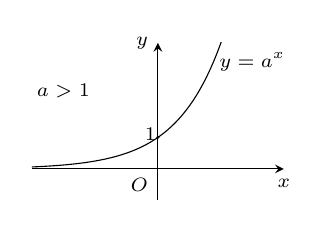
\begin{tikzpicture}[>=stealth,x=1cm,y=1cm,scale=0.4]
			\def\a{2}
			\draw[->] (-4,0) -- (4,0) node[below] {\scriptsize $x$};
			\draw[->] (0,-1) -- (0,4) node[left] {\scriptsize $y$};
			\draw (0,0)node[below left]{\scriptsize $O$};
			\draw (3,4)node[below]{\scriptsize $y=a^x$};
			\draw (-3,3)node[below]{\scriptsize $a>1$};
			\clip (-4,-1)rectangle(4,4);
			\fill (0,1)node[shift={(160:1mm)}]{\scriptsize $1$}circle(1.5pt);
			\draw[thin,samples=150,smooth,domain=-4:4] plot(\x,{\a^(\x)});	
			\end{tikzpicture}}
		
		{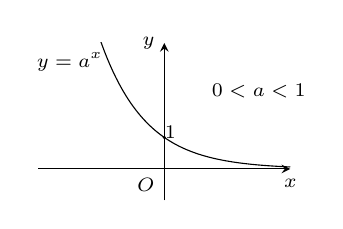
\begin{tikzpicture}[>=stealth,x=1cm,y=1cm,scale=0.4]
			\def\a{1/2}
			\draw[->] (-4,0) -- (4,0) node[below] {\scriptsize $x$};
			\draw[->] (0,-1) -- (0,4) node[left] {\scriptsize $y$};
			\draw (0,0)node[below left]{\scriptsize $O$};
			\draw (-3,4)node[below]{\scriptsize $y=a^x$};
			\draw (3,3)node[below]{\scriptsize $0<a<1$};
			\clip (-4,-1)rectangle(4,4);
			\fill (0,1)node[shift={(40:1mm)}]{\scriptsize $1$}circle(1.5pt);
			\draw[thin,samples=150,smooth,domain=-4:4] plot(\x,{\a^(\x)});	
			\end{tikzpicture}}
	\end{multicols}
	\end{center}
\end{enumerate}

\subsubsection{HÀM SỐ LOGARIT}
1. Định nghĩa\\
Cho số thực dương $a$ khác 1. Hàm số $y=\log_ax$ được gọi là \textbf{hàm số logarit} cơ số $a$.\\
2. Đạo hàm hàm số logarit\\
Định lý 3\\
Hàm số $y=\log_ax\,\,\,(0<a\neq 1)$ có đạo hàm tại mọi $x>0$ và $(\log_ax)'=\dfrac{1}{x\ln a}$\\
Đặc biệt \quad $(\ln x)'=\dfrac{1}{x}$.\\
Chú ý: Đối với hàm hợp $y=\log_au(x)$ ta có $(\log_au)'=\dfrac{u'}{u\ln a}$\\
3. Khảo sát hàm số \quad $y=\log_ax \quad (0<a \ne 1)$
\begin{enumerate} [\indent a)]
	\item Tập xác định: \quad $\mathscr{D}=(0; +\infty)$
	\item Tập giá trị: \quad $\mathscr{T}=\mathbb{R}$
	\item Tính đơn điệu
	\begin{enumerate} [.]
		\item Khi $a>1$ thì hàm số đồng biến trên $(0; +\infty)$.
		\item Khi $0<a<1$ thì hàm số nghịch biến trên $(0; +\infty)$.
	\end{enumerate}
	\item Dạng đồ thị\\
	Đồ thị nhận trục tung làm tiệm cận đứng
	\begin{center}
	\begin{multicols}{3}
		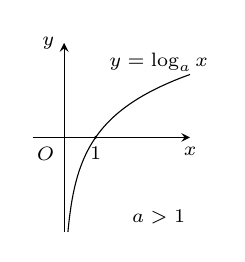
\begin{tikzpicture}[>=stealth,x=1cm,y=1cm,scale=0.4]
		\draw[->] (-1,0) -- (4,0) node[below] {\scriptsize $x$};
		\draw[->] (0,-3) -- (0,3) node[left] {\scriptsize $y$};
		\draw (0,0)node[below left]{\scriptsize $O$};
		\draw (3,3)node[below]{\scriptsize $y=\log_ax$};
		\draw (3,-2)node[below]{\scriptsize $a>1$};
		\clip (-1,-3)rectangle(4,3);
		\fill (1,0)node[below]{\scriptsize $1$}circle(1.5pt);
		\draw[thin,samples=150,smooth,domain=0.1:4] plot(\x,{ln(\x)/ln(2)});	
		\end{tikzpicture}\\
		
		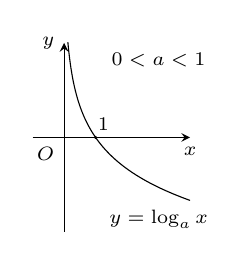
\begin{tikzpicture}[>=stealth,x=1cm,y=1cm,scale=0.4]
		\draw[->] (-1,0) -- (4,0) node[below] {\scriptsize $x$};
		\draw[->] (0,-3) -- (0,3) node[left] {\scriptsize $y$};
		\draw (0,0)node[below left]{\scriptsize $O$};
		\draw (3,-2)node[below]{\scriptsize $y=\log_ax$};
		\draw (3,3)node[below]{\scriptsize $0<a<1$};
		\clip (-1,-3)rectangle(4,3);
		\fill (1,0)node[shift={(60:2mm)}]{\scriptsize $1$}circle(1.5pt);
		\draw[thin,samples=150,smooth,domain=0.1:4] plot(\x,{ln(\x)/ln(1/2)});
		\end{tikzpicture}
	\end{multicols}
	\end{center}
\end{enumerate}

Bảng đạo hàm của các hàm số lũy thừa, mũ, logarit
\begin{center}
	\begin{tabular}{|l|l|}
		\hline 
		Đạo hàm hàm số sơ cấp & Đạo hàm hàm số hợp\\ 
		\hline 
		$\left(a^x\right)'=a^x\cdot \ln a$ & $\left(a^u\right)'=a^u\cdot \ln u \cdot u'$\\ 
		\hline 
		$\left(\mathrm{e}^x\right)'=\mathrm{e}^x$ & $\left(\mathrm{e}^u\right)'=\mathrm{e}^u \cdot u'$\\
		\hline
		$\left(\log_a{|x|}\right)=\dfrac{1}{x\cdot \ln a}$ & $\left(\log_a{|u|}\right)=\dfrac{u'}{u\cdot \ln a}$\\
		\hline
		$\left(\ln |x|\right)'=\dfrac{1}{x}$ & $\left(\ln |u|\right)'=\dfrac{u'}{u}$\\
		\hline
	\end{tabular}
\end{center}

\subsection{Phân loại và phương pháp giải bài tập}
\begin{dang}{Tìm tập xác định của hàm số}
\end{dang}
\subsubsection{Các ví dụ}
\begin{vd}%Ví dụ 1.%[2D2Y4-1]
	Tìm tập xác định của hàm số $y=(x-1)^{\tfrac{1}{5}}$.
	\loigiai{
		Hàm số xác định khi \quad $x-1>0\Leftrightarrow x>1$.\\
		Vậy tập xác định \quad $\mathscr{D}=(1;+\infty)$.}
\end{vd}
\begin{vd}%Ví dụ 2.%[2D2Y4-1]
	Tìm tập xác định của hàm số $f(x)=\log_{\sqrt{2}}{\sqrt{x+1}}-\log_{\tfrac{1}{2}}(3-x)-\log_3(x-1)^3$.
	\loigiai{
		Điều kiện \quad $\heva{&x+1>0\\&3-x>0\\&x-1>0} \Leftrightarrow \heva{&x>-1\\&x<3\\&x>1} \Leftrightarrow 1<x<3$.\\
		Vậy tập xác định \quad $\mathscr{D}=(1;3)$.}
\end{vd}
\begin{vd}%Ví dụ 3.%[2D2B4-1]
	Tìm tập xác định của hàm số $y=\sqrt{2-\ln(\mathrm{e}x)}$.
	\loigiai{
		Điều kiện \quad $\heva{&\mathrm{e}x>0\\&2-\ln(\mathrm{e}x)\geq 0}\Leftrightarrow\heva{&x>0\\&\ln(\mathrm{e}x)\leq 2}\Leftrightarrow\heva{&x>0\\&1+\ln x\leq 2}\Leftrightarrow\heva{&x>0\\&x\leq \mathrm{e}} \Leftrightarrow 0<x\leq \mathrm{e}$.\\
		Vậy tập xác định \quad $\mathscr{D}=(0;\mathrm{e}]$.}
\end{vd}
\begin{vd}%Ví dụ 4.%[2D2B4-1]
	Tìm tập xác định của hàm số $f(x)=x^x+\ln\dfrac{\mathrm{e}^{2x}+4\mathrm{e}^x+5}{1-x}$.
	\loigiai{
		Điều kiện \quad $\heva{&x>0\\&\dfrac{\mathrm{e}^{2x}+4\mathrm{e}^x+5}{1-x}>0} \Leftrightarrow \heva{&x>0\\&x<1} \Leftrightarrow 0<x<1$.\\
		Vậy tập xác định \quad $\mathscr{D}=(0;1)$.}
\end{vd}
\begin{vd}%Ví dụ 5.%[2D2K4-1]
	Tìm tất cả các giá trị của tham số $m$ sao cho hàm số $y=\dfrac{1}{\sqrt{\log_3(x^2-2x+3m)}}$ có tập xác định là $\mathbb{R}$.
	\loigiai{
		Hàm số có tập xác định $\mathbb{R}$ $\Leftrightarrow \forall x \in \mathbb{R}: \heva{&x^2-2x+3m>0\\&\log_3(x^2-2x+3m)>0}$\\
		$\Leftrightarrow \heva{&x^2-2x+3m>0\\&x^2-2x+3m>1} \Leftrightarrow x^2-2x+3m>1 \Leftrightarrow x^2-2x+3m-1>0$\\
		$\Leftrightarrow \Delta'=(-1)^2-1\cdot(3m-1)<0 \Leftrightarrow m>\dfrac{2}{3}$.\\
		Vậy $m>\dfrac{2}{3}$ là giá trị cần tìm.}
\end{vd}

\subsubsection{Câu hỏi trắc nghiệm}
\begin{ex}%Câu 1.%[2D2Y4-1]
	Tập xác định của hàm số $y=(x-5)^{\sqrt{3}}$ là
	\choice
	{$(-\infty;5)$}
	{$\mathbb{R}\setminus\{5\}$}
	{$[5;+\infty)$}
	{\True $(5;+\infty)$}
	\loigiai{
		Vì $\sqrt{3}$ không nguyên nên hàm số $y=(x-5)^{\sqrt{3}}$ xác định $\Leftrightarrow x-5>0\Leftrightarrow x>5$.\\
		Tập xác định của hàm số là \quad $\mathscr{D}=(5;+\infty)$.}
\end{ex}
\begin{ex}%Câu 2.%[2D2Y4-1]
	Tập xác định của hàm số $y=\dfrac{1}{\sqrt{2-x}}+\ln(x-1)$ là 
	\choice
	{$\mathscr{D}=[1; 2]$}
	{$\mathscr{D}=(1;+\infty)$}
	{\True $\mathscr{D}=(1; 2)$}
	{$\mathscr{D}=(0;+\infty)$}
	\loigiai{
		Điều kiện \quad  $\heva{&2-x>0\\&x-1>0}\Leftrightarrow 1<x<2$.\\
		Vậy tập xác định \quad $\mathscr{D}=(1;2)$.}
\end{ex}
\begin{ex}%Câu 3.%[2D2Y4-1]
	Tập xác định của hàm số  $y=\ln\left(-x^2+5x-6\right)$ là
	\choice
	{$(-\infty; 2)\cup(3;+\infty)$}
	{\True $(2; 3)$}
	{$(-\infty; 2]\cup[3;+\infty)$}
	{$[2; 3]$}
	\loigiai{
		Điều kiện xác định $-x^2+5x-6>0\Leftrightarrow x\in(2; 3)$.\\
		Vậy tập xác định \quad $\mathscr{D}=(2;3)$.}
\end{ex}
\begin{ex}%Câu 4.%[2D2Y4-1]
	Tìm tập xác định của hàm số $y=\left(4x^2-1\right)^{-4}$. 
	\choice
	{$\left(-\dfrac{1}{2};\dfrac{1}{2}\right)$}
	{$(0;+\infty)$}
	{$\mathbb{R}$}
	{\True $\mathbb{R}\setminus\left\{-\dfrac{1}{2};\dfrac{1}{2}\right\}$}
	\loigiai{
		Do $\alpha=-4$ là số nguyên âm nên điều kiện xác định là $4x^2-1\neq 0\Leftrightarrow\heva{&x\neq-\dfrac{1}{2}\\&x\neq\dfrac{1}{2}.}$ \\
		Vậy tập xác định \quad $\mathscr{D}=\mathbb{R}\setminus\left\{-\dfrac{1}{2};\dfrac{1}{2}\right\}$.}
\end{ex}
\begin{ex}%Câu 5.%[2D2Y4-1]
	Tập xác định của hàm số $y=\log_2\left(3-2x-x^2\right)$ là 
	\choice
	{$\mathscr{D}=(-1;3)$}
	{$\mathscr{D}=(0;1)$}
	{$\mathscr{D}=(-1;1)$}
	{\True $\mathscr{D}=(-3;1)$}
	\loigiai{
		Hàm số $y=\log_2\left(3-2x-x^2\right)$ xác định khi $3-2x-x^2>0\Leftrightarrow-3<x<1$.\\
		Vậy tập xác định \quad  $\mathscr{D}=(-3;1)$.}
\end{ex}
\begin{ex}%Câu 6.%[2D2B4-1]
	Tìm tập xác định $\mathscr{D}$ của hàm số $y=\log_x\left(\dfrac{2x}{3-x}\right)$ là
	\choice
	{\True $\mathscr{D}=(0;3)\setminus\{1\}$}
	{$\mathscr{D}=(0;3)$}
	{$\mathscr{D}=(1;3)$}
	{$\mathscr{D}=(0;1)$}
	\loigiai{
		Điều kiện \quad $\heva{&0<x\neq 1\\&\dfrac{2x}{3-x}>0}\Leftrightarrow\heva{&0<x\neq 1\\&3-x>0}\Leftrightarrow\heva{&0<x\neq 1\\&x<3}\Leftrightarrow\heva{&0<x<3\\&x\neq 1.}$ \\
		Vậy $\mathscr{D}=(0;3)\setminus\{1\}$.}
\end{ex}
\begin{ex}%Câu 7.%[2D2B4-1]
	Tìm tập xác định $\mathscr{D}$ của hàm số $y=\log_x\left(\dfrac{2x}{3-x}\right)$ là
	\choice
	{\True $\mathscr{D}=(0;3)\setminus\{1\}$}
	{$\mathscr{D}=(0;3)$}
	{$\mathscr{D}=(1;3)$}
	{$\mathscr{D}=(0;1)$}
	\loigiai{
		Điều kiện \quad $\heva{&0<x\neq 1\\&\dfrac{2x}{3-x}>0}\Leftrightarrow\heva{&0<x\neq 1\\&3-x>0}\Leftrightarrow\heva{&0<x\neq 1\\&x<3}\Leftrightarrow\heva{&0<x<3\\&x\neq 1.}$ \\
		Vậy $\mathscr{D}=(0;3)\setminus\{1\}$.}
\end{ex}
\begin{ex}%Câu 8.%[2D2Y4-1]
	Tìm tập xác định của hàm số $f(x)=\left(1+\sqrt{x-1}\right)^{\sqrt{3}}$. 
	\choice
	{$\mathscr{D}=\mathbb{R}$}
	{\True $\mathscr{D}=[1;+\infty)$}
	{$\mathscr{D}=(0;+\infty)$}
	{$\mathscr{D}=\mathbb{R}\setminus\{1\}$}
	\loigiai{
		$f(x)$ là hàm số lũy thừa với số mũ không nguyên nên cơ số phải là số dương.\\
		Điều kiện xác định \quad $\heva{&x-1\geq 0\\&1+\sqrt{x-1}>0}\Leftrightarrow x\geq 1$.\\
		Vậy tập xác định \quad $\mathscr{D}=[1;+\infty)$.}
\end{ex}
\begin{ex}%Câu 9.%[2D2Y4-1]
	Tìm tập xác định $\mathscr{D}$ của hàm số $y=\left(3x^2-1\right)^{\tfrac{1}{3}}$. 
	\choice
	{$\mathscr{D}=\left(-\infty;-\dfrac{1}{\sqrt{3}}\right]\cup\left[\dfrac{1}{\sqrt{3}};+\infty\right)$}
	{\True $\mathscr{D}=\left(-\infty;-\dfrac{1}{\sqrt{3}}\right)\cup\left(\dfrac{1}{\sqrt{3}};+\infty\right)$}
	{$\mathscr{D}=\mathbb{R}\setminus\left\{\pm\dfrac{1}{\sqrt{3}}\right\}$}
	{$\mathscr{D}=\mathbb{R}$}
	\loigiai{
		Hàm số xác định khi và chỉ khi $3x^2-1>0\Leftrightarrow\hoac{&x <-\dfrac{1}{\sqrt{3}}\\&x>\dfrac{1}{\sqrt{3}}.}$ \\
		Vậy tập xác định \quad  $\mathscr{D}=\left(-\infty;-\dfrac{1}{\sqrt{3}}\right)\cup\left(\dfrac{1}{\sqrt{3}};+\infty\right)$.}
\end{ex}
\begin{ex}%Câu 10.%[2D2Y4-1]
	Tìm tập xác định của hàm số $y=\log_2\left(2^{3-6x}-1\right)$. 
	\choice
	{\True $\mathscr{D}=\left(-\infty;\dfrac{1}{2}\right)$}
	{$\mathscr{D}=\left(-\infty;-\dfrac{1}{2}\right)$}
	{$\mathscr{D}=\mathbb{R}$}
	{$\mathscr{D}=\left(\dfrac{1}{2};+\infty\right)$}
	\loigiai{
		Điều kiện xác định \quad $2^{3-6x}-1>0\Leftrightarrow 3-6x>0\Leftrightarrow x<\dfrac{1}{2}$.\\
		Vậy tập xác định \quad $\mathscr{D}=\left(-\infty;\dfrac{1}{2}\right)$.}
\end{ex}
\begin{ex}%Câu 11.%[2D2B4-1]
	Điều kiện xác định của hàm số $y=\ln\left(x-2-\sqrt{x^2-3x-10}\right)$ là
	\choice
	{$5\leq x\leq 14$}
	{$2<x<14$}
	{$2\leq x<14$}
	{\True $5\leq x<14$}
	\loigiai{
		Điều kiện xác định $x-2-\sqrt{x^2-3x-10}>0\Leftrightarrow\sqrt{x^2-3x-10}<x-2$\\
		$\Leftrightarrow \heva{&x-2>0\\&x^2-3x-10\geq 0\\&x^2-3x-10<x^2-4x+4} \Leftrightarrow \heva{&x>2\\&x\leq-2\vee x\geq 5\\&x<14} \Leftrightarrow 5\leq x<14 $.}
\end{ex}
\begin{ex}%Câu 12.%[2D2B4-1]
	Tìm tất cả các giá trị thực của tham số $m$ để hàm số $y=\log_{2017}(mx-m+2)$ xác định trên $[1;+\infty)$. 
	\choice
	{\True $m\geq 0$}
	{$m\geq-1$}
	{$m\leq-1$}
	{$m\leq 0$}
	\loigiai{
		Hàm số xác định trên $[1;+\infty)$ khi $mx-m+2>0$ với mọi $x\in[1;+\infty)$.\\
		Xét bất phương trình $mx-m+2>0\Leftrightarrow mx>m-2 \quad (1)$.
		\begin{enumerate}
			\item Nếu $m=0$ thì $(1)$ trở thành  $ 0\cdot x>-2$ (luôn đúng với mọi $x \in [1;+\infty)$).
			\item Nếu $m>0$ thì $(1)\Leftrightarrow x>\dfrac{m-2}{m}=1-\dfrac{2}{m}$.\\
			Khi đó $(1)$ thỏa mãn với $x\ge 1$ vì $1-\dfrac{2}{m}<1$ khi $m>0$.
			\item Nếu $m<0$ thì $(1)\Leftrightarrow x<\dfrac{m-2}{m}$.\\
			Khi đó $(1)$ không thỏa mãn với mọi $x\ge 1$.
		\end{enumerate}
		Vậy $m\ge 0$ là giá trị cần tìm.}
\end{ex}
\begin{ex}%Câu 13.%[2D2B4-1]
	Tìm tất cả các giá trị của $m$ để hàm số $y=\log_3\left(-x^2+mx+2m+1\right)$ xác định với mọi $x\in(1;2)$ 
	\choice
	{$m\geq-\dfrac{1}{3}$}
	{\True $m\geq\dfrac{3}{4}$}
	{$m>\dfrac{3}{4}$}
	{$m <-\dfrac{1}{3}$}
	\loigiai{
		Hàm số xác định với mọi $x\in(1;2)$ khi $-x^2+mx+2m+1>0,\,\,\forall x\in(1;2)$\\
		$\Leftrightarrow f(x)=x^2-mx-2m-1<0,\,\,\forall x\in(1;2)$ \\
		$\Leftrightarrow f(x)=0 $ có hai nghiệm thỏa $x_1\leq 1<2\leq x_2$ \\
		$\Leftrightarrow\heva{&f(1)\leq 0\\&f(2)\leq 0}\Leftrightarrow\heva{&-3m\leq 0\\&3-4m\leq 0}\Leftrightarrow m\geq\dfrac{3}{4} $.}
\end{ex}
\begin{ex}%Câu 14.%[2D2B4-1]
	Hàm số $y=\log_2\left(4^x-2^x+m\right)$ có tập xác định là $\mathbb{R}$ khi
	\choice
	{$m<\dfrac{1}{4}$}
	{$m>0$}
	{$m\geq\dfrac{1}{4}$}
	{\True $m>\dfrac{1}{4}$}
	\loigiai{
		Điều kiện \quad $4^x-2^x+m>0$.\\
		Hàm số đã cho có tập xác định là $\mathbb{R}$ khi và chỉ khi $4^x-2^x+m>0 \quad (1) \quad \forall x \in \mathbb{R}$.\\
		Đặt $t=2^x \quad (t>0)$, khi đó bất phương trình $(1)$ trở thành $t^2-t+m>0 \quad \forall t>0$.\\
		Xét hàm số $f(t)=t^2-t,\,\,\, \forall t>0$.\\
		Ta có $f'(t)=2t-1; \quad f'(t)=0\Leftrightarrow t=\dfrac{1}{2}$.\\
		Lập bảng biến thiên ta tìm được $\min\limits_{(0;+\infty)} f(t)=f\left(\dfrac{1}{2}\right)=-\dfrac{1}{4}$.\\
		Để bất phương trình $t^2-t+m>0 \quad \forall t>0$ thì $-m <-\dfrac{1}{4}\Leftrightarrow m>\dfrac{1}{4}$.}
\end{ex}
\begin{ex}%Câu 15.%[2D2B4-1]
	Tập xác định $\mathscr{D}$ của hàm số $y=\log_{x-1}{\dfrac{x}{2-x}}$ là 
	\choice
	{$(1; +\infty)$}
	{$(0;1)$}
	{$(2;+\infty)$}
	{\True $(1;2)$}
	\loigiai{
		Điều kiện \quad $\heva{&0<x-1\neq 1\\&\dfrac{x}{2-x}>0}\Leftrightarrow\heva{&x>1\\&x\neq 2\\&x\in(0;2)}\Leftrightarrow x\in(1;2)$.}
\end{ex}
\begin{ex}%Câu 16.%[2D2B4-1]
	Hàm số $y=\ln|1-\sin x|$ có tập xác định là 
	\choice
	{\True $\mathbb{R}\setminus\left\{\dfrac{\pi}{2}+k2\pi\right\}$}
	{$\mathbb{R}\setminus\{\pi+k2\pi\}$}
	{$\mathbb{R}\setminus\left\{\dfrac{\pi}{3}+k2\pi\right\}$}
	{$\mathbb{R}$}
	\loigiai{
		Điều kiện
		$\left|1-\sin x\right|>0 \Leftrightarrow 1-\sin x\neq 0 \Leftrightarrow\sin x\neq 1 \Leftrightarrow x\neq\dfrac{\pi}{2}+k2\pi, k\in\mathbb{Z}$.\\
		Vậy tập xác định \quad $\mathscr{D}=\mathbb{R}\setminus \left\{\dfrac{\pi}{2}+k2\pi\right\}$ .}
\end{ex}
\begin{ex}%Câu 17.%[2D2B4-1]
	Tìm $m$ để hàm số $y=2x+2017+\ln(x^2-2mx+4)$ có tập xác định $\mathscr{D}=\mathbb{R}$ 
	\choice
	{$m=2$}
	{$m>2$}
	{$\hoac{&m<-2\\&m>2}$}
	{\True $\heva{&m<2\\&m>-2}$}
	\loigiai{
		Hàm số có TXĐ $\mathscr{D}=\mathbb{R} \Leftrightarrow x^2-2mx+4>0,\,\,\,\forall x \in \mathbb{R} \Leftrightarrow \Delta'<0 \Leftrightarrow m^2-4<0 \Leftrightarrow m \in (-2; 2)$.}
\end{ex}
\begin{ex}%Câu 18.%[2D2B4-1]
	Tìm tất cả các giá trị thực của tham số $m$ để hàm số $y=\log(x^2-2x-m+1)$ có tập xác định là $\mathbb{R}$ 
	\choice
	{$m \ge 0$}
	{\True $m<0$}
	{$m \le 2$}
	{$m>2$}
	\loigiai{
		Ycbt $\Leftrightarrow x^2-2x-m+1>0,\,\,\,\forall x \in \mathbb{R} \Leftrightarrow \heva{&a>0\\&\Delta'=1+m-1<0} \Leftrightarrow m<0$.}
\end{ex}
\begin{ex}%Câu 19.%[2D2B4-1]
	Hàm số $y=\log_2(4^x-2^x+m)$ có tập xác định $\mathscr{D}=\mathbb{R}$ khi 
	\choice
	{$m \ge \dfrac{1}{4}$}
	{\True $m > \dfrac{1}{4}$}
	{$m<\dfrac{1}{4}$}
	{$m>0$}
	\loigiai{
		Hàm số có tập xác định $\mathscr{D}=\mathbb{R}$ khi và chỉ khi $4^x-2^x+m>0,\,\,\,\forall x \in \mathbb{R} \quad (*)$.\\
		Đặt $t=2^x>0$ khi đó $(*) \Leftrightarrow t^2-t+m>0,\,\,\,\forall t>0 \Leftrightarrow m>t-t^2,\,\,\,\forall t>0 \Leftrightarrow m> \max\limits_{x \in (0;+\infty)}(t-t^2)$.\\
		Ta có \quad $t-t^2=\dfrac{1}{4}-\left(\dfrac{1}{2}-t\right)^2 \le \dfrac{1}{4}$ suy ra $m>\dfrac{1}{4}$.}
\end{ex}
\begin{ex}%Câu 20.%[2D2K4-1]
	Có bao nhiêu giá trị nguyên dương của tham số $m$ để hàm số $y=\log_2\left(\dfrac{4^x+2^{x+1}+10}{2^x+1}-m\right)$ có tập xác định $\mathscr{D}=\mathbb{R}$?
	\choice
	{$1$}
	{\True $5$}
	{$10$}
	{$13$}
	\loigiai{
		Ycbt $\Leftrightarrow \dfrac{4^x+2^{x+1}+10}{2^x+1}-m>0,\,\,\,\forall x \in \mathbb{R} \Leftrightarrow m<\dfrac{4^x+2^{x+1}+10}{2^x+1},\,\,\,\forall x \in \mathbb{R} \Leftrightarrow m<\min\limits_{x \in \mathbb{R}}\dfrac{4^x+2^{x+1}+10}{2^x+1}$.\\
		Ta có \quad $\dfrac{4^x+2^{x+1}+10}{2^x+1}=\dfrac{\left(2^x+1\right)^2+9}{2^x+1}=2^x+1+\dfrac{9}{2^x+1}\ge 2\sqrt{9}=6$.\\
		Suy ra $m<6$. Vậy có $5$ giá trị nguyên dương của $m$.}
\end{ex}

\Closesolutionfile{ans}
%\DAPAN
%\inputansbox{10}{ans/ans-2D2-4(1)}
\Opensolutionfile{ans}[ans/ans-2D2-4(2)]
\begin{dang}{Đạo hàm của hàm số mũ, hàm số logarit}
\end{dang}
Các bài toán tìm đạo hàm của hàm số mũ, đạo hàm hàm số logarit, các bài toán chứa tham số, giải các phương trình, bất phương trình liên quan đến đạo hàm hàm số mũ, hàm số logarit…
\subsubsection{Các ví dụ}
\begin{vd}%[2D2B4-2]%Ví dụ 1.
	Tìm đạo hàm của hàm số $y=e^{\cos 2 x}$ tại $x=\dfrac{\pi}{6}$.
	\loigiai{
		Ta có $y'=(\cos 2 x)' \cdot e^{\cos 2 x}=-2 \sin 2 x e^{\cos 2 x} \Rightarrow y'\left(\dfrac{\pi}{6}\right)=-2 \sin \dfrac{\pi}{3} e^{\cos \frac{\pi}{3}}=-\sqrt{3 e}$}
%<MyLT>
\end{vd}
\begin{vd}%[2D2B4-2]%Ví dụ 2.
	Tìm đạo hàm của hàm số $y=\log_8\left( x^2-3x+8 \right)$.
	\loigiai{
		Ta có $y'=\dfrac{\left(x^{2}-3 x+8\right)'}{\left(x^{2}-3 x+8\right) \cdot \ln 8}=\dfrac{2 x-3}{\left(x^{2}-3 x+8\right) \cdot \ln 8}$}
%<MyLT>
\end{vd}
\begin{vd}%[2D2B4-2] %Ví dụ 3.
	Cho hàm số $y=\ln \dfrac{1}{x+1}$. Chứng minh $xy'+1=e^{y}$.
	\loigiai{
		Ta có $y'=\left(\dfrac{1}{x+1}\right)' \cdot \dfrac{1}{\dfrac{1}{x+1}}=-\dfrac{1}{(x+1)^{2}}(x+1)=-\dfrac{1}{x+1}$ \\
		Vậy $xy'+1=-\frac{x}{x+1}+1=\dfrac{1}{x+1}$ và $e^{y}=e^{\ln \dfrac{1}{x+1}}=\dfrac{1}{x+1} \Rightarrow x y'+1=e^{y}$}
\end{vd}
\begin{vd}%[2D2B4-2] %Ví dụ 4.
	Cho $f(x)=2^{\frac{x-1}{x+1}}$. Tìm giá trị $f'(0)$.
	\loigiai{
		$f'(x)=2^{\frac{x-1}{x+1}} \cdot \ln 2 \cdot\left(\dfrac{x-1}{x+1}\right)'=\dfrac{2}{(x+1)^{2}} \cdot 2^{\frac{x-1}{x+1}} \cdot \ln 2 \Rightarrow f'(0)=2 \cdot 2^{-1} \cdot \ln 2=\ln 2$}
\end{vd}
\begin{vd}%[2D2B4-2] %Ví dụ 5.
	Tìm đạo hàm của hàm số $y=\ln (x+\sqrt{x^{2}+1})$.
	\loigiai{
		Ta có $y'=\dfrac{(x+\sqrt{x^{2}+1})'}{x+\sqrt{x^{2}+1}}=\dfrac{1+\dfrac{x}{\sqrt{x^{2}+1}}}{x+\sqrt{x^{2}+1}}=\dfrac{1}{\sqrt{x^{2}+1}}$}
\end{vd}
\subsubsection{Câu hỏi trắc nghiệm}
\begin{ex}%[2D2Y4-2] %Câu 1.
	Tính đạo hàm của hàm số $f(x)=\log_2(x+1)$ 
	\choice
	{$f'(x)=\dfrac{1}{x+1}$}
	{$f'(x)=log_2(x+1)$}
	{\True $f'(x)=\dfrac{1}{(x+2)\ln2}$}
	{$f'(x)=0$}
	\loigiai{
		Ta có: $f'(x)=\dfrac{1}{(x+2)\ln2}$}
\end{ex}
\begin{ex}%[2D2Y4-2] %Câu 2.
	Tính đạo hàm của hàm số $y=13^x$\\. 
	\choice
	{$y'=x.13^{x-1}$}
	{\True $y'=13^{x}\ln 13$}
	{$y'=13^x$}
	{$y'=\dfrac{13^x}{\ln13}$}
	\loigiai{
		Áp dụng công thức đạo hàm $(a^x)=a^x\ln a$ ta được $y'=13^{x}\ln 13$ }
\end{ex}
\begin{ex}%[2D2Y4-2] %Câu 3.
	Tính đạo hàm của hàm số $y=2^{x^2}$
	\choice
	{$y'=\dfrac{x.2^{1+x^2}}{\ln2}$}
	{\True $y'=x.2^{1+x^2}.\ln2$}
	{$y'=2^x.\ln2^x$}
	{$y'=\dfrac{x.2^{1+x}}{\ln2}$}
	\loigiai{
		Áp dụng công thức đạo hàm $(a^u)'=u'\cdot a^u\ln a$ ta được $y'=2x.2^{x^2}.\ln2=x.2^{1+x^2}.\ln2$}
\end{ex}
\begin{ex}%[2D2Y4-2] %Câu 4.
	Tính đạo hàm của hàm số $y=e^{\sqrt{2x}}$
	\choice
	{\True $y'=\dfrac{e^{\sqrt{2x}}}{2\sqrt{2x}}$}
	{$y'=\dfrac{e^{\sqrt{x}}}{\sqrt{2x}}$}
	{$y'=\dfrac{e^{\sqrt{2x}}}{\sqrt{2x}}$}
	{$y'=\sqrt{2x}.e^{\sqrt{2x}}$}
	\loigiai{
		Áp dụng công thức đạo hàm $(\mathrm{e}^u)'=u'\cdot\mathrm{e}^u$ ta được $y'=\dfrac{e^{\sqrt{2x}}}{2\sqrt{2x}}$.}
\end{ex}
\begin{ex}%[2D2Y4-2] %Câu 5.
	Tìm đạo hàm của hàm số $y=2x^2-\dfrac{1}{x}+\sin 2x+3^x+1$. 
	\choice
	{$y'=4x-\dfrac{1}{x^2}+\cos 2x+3^x\ln 3$}
	{\True $y'=4x+\dfrac{1}{x^2}+2\cos 2x+3^x\ln 3$}
	{$y'=4x+\dfrac{1}{x^2}+2\cos 2x+\dfrac{3^x}{\ln 3}$}
	{$y'=2x+\dfrac{1}{x^2}+2\cos 2x+3^x$}
	\loigiai{
		$y'=4x+\dfrac{1}{x^2}+2\cos 2x+3^x\ln 3$.}
\end{ex}
\begin{ex}%[2D2B4-2] %Câu 6.
	Cho hàm số $f(x)=\ln^2\left(x^2-2x+4\right)$. Tìm các giá trị của $x$ để $f'(x)>0$. 
	\choice
	{$x\neq 1$}
	{$x>0$}
	{\True $x>1$}
	{$\forall x$}
	\loigiai{
		Tập xác định: $\mathscr{D}=\mathbb{R}$.\\
		$f'(x)=\dfrac{4x-4}{x^2-2x+4}.\ln\left(x^2-2x+4\right)$.\\
		\textbf{Nhận xét:} $\ln\left(x^2-2x+4\right)>0,\forall x\in\mathbb{R}$ do $x^2-2x+4>1,\forall x\in\mathbb{R}$.\\
		Do đó $f'(x)>0\Leftrightarrow 4x-4>0\Leftrightarrow x>1$.}
\end{ex}
\begin{ex}%[2D2B4-2] %Câu 7.
	Cho hàm số $y=\ln\left(\mathrm{e}^x+m^2\right)$. Với giá trị nào của $m$ thì $y'(1)=\dfrac{1}{2}$. 
	\choice
	{$m=e$}
	{$m=-e$}
	{$m=\dfrac{1}{e}$}
	{\True $m=\pm\sqrt{e}$}
	\loigiai{
		Ta có $y'=\dfrac{\mathrm{e}^x}{\mathrm{e}^x+m^2}\Rightarrow y'(1)=\dfrac{e}{e+m^2}$.\\
		Khi đó $y'(1)=\dfrac{1}{2}\Leftrightarrow\dfrac{e}{e+m^2}=\dfrac{1}{2}\Leftrightarrow 2e=e+m^2\Leftrightarrow m=\pm\sqrt{e}$.}
\end{ex}
\begin{ex}%[2D2B4-2] %Câu 8.
	Đạo hàm của hàm số $y=\log_{3x}(5x+2)$ là
	\choice
	{$y'=\dfrac{1}{(5x+2)\ln(3x)}$}
	{$y'=\dfrac{1}{(5x+2)\ln(2x)}$}
	{\True $y'=\dfrac{5x\ln(3x)-(5x+2)\ln(5x+2)}{x(5x+2)[\ln(3x)]^2}$}
	{$y'=\dfrac{5x\ln(3x)-(5x+2)\ln(5x+2)}{x(5x+2)^2[\ln(3x)]^2}$}
	\loigiai{
		$y=\log_{3x}(5x+2)=\dfrac{\ln(5x+2)}{\ln(3x)}$.\\
		$y'=\dfrac{\dfrac{5}{5x+2}\ln(3x)-\dfrac{3}{3x}\ln (5x+2)}{[\ln(3x)]^2} =\dfrac{5x\ln(3x)-(5x+2)\ln (5x+2)}{x(5x+2)[\ln(3x)]^2}$.}
\end{ex}
\begin{ex}%[2D2B4-2] %Câu 9.
	Cho hàm số $y=\dfrac{\mathrm{e}^x}{x}$. Chọn mệnh đề đúng trong các mệnh đề sau: 
	\choice
	{$y'+xy''=\mathrm{e}^x,\forall x\neq 0$}
	{$y'+xy''=-\mathrm{e}^x,\forall x\neq 0$}
	{\True $2y'+xy''=\mathrm{e}^x,\forall x\neq 0$}
	{$2y'+xy''=-\mathrm{e}^x,\forall x\neq 0$}
	\loigiai{		
		Ta có: $y'=\dfrac{\mathrm{e}^x\cdot x-\mathrm{e}^x}{x^2}$; $y''=\dfrac{\left(\mathrm{e}^x+x\mathrm{e}^x-\mathrm{e}^x\right)x^2-2x\left(x\mathrm{e}^x-\mathrm{e}^x\right)}{x^4} =\dfrac{x^2\mathrm{e}^x-2x\mathrm{e}^x+2\mathrm{e}^x}{x^3}$.\\
		$2y'+xy''=\dfrac{2x\mathrm{e}^x-2\mathrm{e}^x}{x^2}+\dfrac{x^2\mathrm{e}^x-2x\mathrm{e}^x+2\mathrm{e}^x}{x^2}=\mathrm{e}^x$.}
\end{ex}
\begin{ex}%[2D2B4-2] %Câu 10.
	Tính đạo hàm của hàm số $y=\dfrac{x+2}{9^x}$ 
	\choice
	{$y'=\dfrac{1+2(x+2)\ln 3}{3^{2x}}$}
	{\True $y'=\dfrac{1-2(x+2)\ln 3}{3^{2x}}$}
	{$y'=\dfrac{1+(x+2)\ln 3}{3^{2x}}$}
	{$y'=\dfrac{1-(x+2)\ln 3}{3^{2x}}$}
	\loigiai{
		Ta có: $y'=\left(\dfrac{x+2}{9^x}\right)'=\dfrac{(x+2)'{\cdot 9}^x-(9^x)'(x+2)}{9^{2x}}=\dfrac{9^x-9^x\ln 9(x+2)}{9^{2x}}$.\\
		$y'=\dfrac{9^x-9^x\ln 9(x+2)}{9^{2x}}=\dfrac{1-2(x+2)\ln 3}{3^{2x}}$.}
\end{ex}
\begin{ex}%[2D2B4-2] %Câu 11.
	Cho hàm số $f(x)=\ln^2\left(x^2-2x+5\right)$. Tìm các giá trị của $x$ để $f'(x)>0$. 
	\choice
	{$x>0$}
	{$x\neq 1$}
	{$x\in\mathbb{R}$}
	{\True $x>1$}
	\loigiai{
		Tập xác định $\mathscr{D}=\mathbb{R}$.\\
		Ta có $f'(x)=2\ln\left(x^2-2x+5\right)\cdot\left(\ln\left(x^2-2x+5\right)\right)'=2\ln\left(x^2-2x+5\right)\cdot\dfrac{2x-2}{x^2-2x+5}$.\\
		Do đó $f'(x)>0\Leftrightarrow\ln\left(x^2-2x+5\right)\cdot\dfrac{x-1}{(x-1)^2+4}>0$ \\
		$ \Leftrightarrow(x-1)\cdot\ln\left((x-1)^2+4\right)>0 $.\\
		Mặt khác $(x-1)^2+4\geq 4\Rightarrow\ln\left((x-1)^2+4\right)\geq\ln 4>0$ nên $f'(x)>0\Leftrightarrow x>1$.}
\end{ex}
\begin{ex}%[2D2K4-2] %Câu 12.
	Cho hàm số $f(x)=\dfrac{2x^3}{3}+\ln x$. Giá trị nhỏ nhất của hàm số $g(x)=\dfrac{1}{x}f'(x)$ là
	\choice
	{$3$}
	{$2$}
	{$1$}
	{\True Giá trị khác}
	\loigiai{
		TXĐ: $\mathscr{D}=(0;+\infty)$.\\
		$f'(x)=x^2+\dfrac{1}{x}$.\\
		$g(x)=\dfrac{1}{x}f'(x)=x+\dfrac{1}{x^2}\Rightarrow g'(x)=1-\dfrac{2}{x^3}=0\Leftrightarrow x=\sqrt[3]{2}$.\\
		Bảng biến thiên: 
		\begin{center}
			
\begin{tikzpicture}
			\tkzTabInit[nocadre=false,lgt=1.2,espcl=2.5,deltacl=0.6]
			{$x$ /0.6,$y'$ /0.6,$y$ /2}
			{$0$,$\sqrt[3]{2}$,$+\infty$}
			\tkzTabLine{,-,$0$,+,}
			\tkzTabVar{+/, -/$\sqrt[3]{2}+\dfrac{1}{\sqrt[3]{4}}$,+/}
			\end{tikzpicture}
		\end{center}	
	}
\end{ex}
\begin{ex}%[2D2K4-2] %Câu 13.
	Tính đạo hàm cấp $2018$ của hàm số $y=\mathrm{e}^{2x}$. 
	\choice
	{$y^{(2018)}=2^{2017}\cdot\mathrm{e}^{2x}$}
	{\True $y^{(2018)}=2^{2018}\cdot\mathrm{e}^{2x}$}
	{$y^{(2018)}=\mathrm{e}^{2x}$}
	{$y^{(2018)}=2^{2018}\cdot x\cdot\mathrm{e}^{2x}$}
	\loigiai{
		$y'=2\cdot\mathrm{e}^{2x}$;\\
		$y''=2^2\cdot\mathrm{e}^{2x}$;\\
		$y^{(3)}=2^3\cdot\mathrm{e}^{2x}$;\\
		….\\
		$y^{(n)}=2^n\cdot\mathrm{e}^{2x} (*)$.\\
		Thật vậy.\\
		Với $n=1$ công thức $(*)$ đúng.\\
		Giả sử $(*)$ đúng với $n=k$, tức là ta có $y^{(k)}=2^k\cdot\mathrm{e}^{2x}$.\\
		Khi đó $y^{(k+1)}=2^k\cdot 2\cdot\mathrm{e}^{2x}=2^{k+1}\cdot\mathrm{e}^{2x}$.\\
		Vậy $(*)$ đúng với mọi $n\in\mathbb{N}$.\\
		Vậy $y^{(2018)}=2^{2018}\cdot\mathrm{e}^{2x}$.}
\end{ex}
\begin{ex}%[2D2K4-2] %Câu 14.
	Cho $f(x)=\dfrac{1}{2}\cdot 5^{2x+1}$; $g(x)=5^x+4x\cdot\ln 5$. Tập nghiệm của bất phương trình $f'(x)>g'(x)$ là
	\choice
	{$x<0$}
	{$x>1$}
	{$0<x<1$}
	{\True $x>0$}
	\loigiai{
		Ta có: $f'(x)=\dfrac{1}{2}\cdot 5^{2x+1}\cdot (2x+1)'\cdot\ln 5=5^{2x+1}\cdot\ln 5$.\\
		Và: $g'(x)=5^x\cdot\ln 5+4\ln 5=\left(5^x+4\right)\ln 5$.\\
		Do đó: $f'(x)>g'(x)\Leftrightarrow 5^{2x+1}\cdot\ln 5>\left(5^x+4\right)\ln 5$\\
		$\Leftrightarrow 5^{2x+1}>5^x+4$
		$\Leftrightarrow 5\cdot 5^{2x}-5^x-4>0$ \\
		$ \Leftrightarrow\hoac{&5^x <-\dfrac{4}{5}(\text{vô nghiệm})\\&5^x>1}\Leftrightarrow 5^x>1\Leftrightarrow x>0 $.\\
		Vậy nghiệm của bất phương trình đã cho là $x>0$.}
\end{ex}
\begin{ex}%[2D2K4-2] %Câu 15.
	Cho hàm số $f(x)=\mathrm{e}^{10x+20}$. Tìm $f^{(2018)}(x)$. 
	\choice
	{$f^{(2018)}(x)=200\cdot\mathrm{e}^{10x+20}$}
	{$f^{(2018)}(x)=10^{2018}\cdot 20^{1009}\cdot\mathrm{e}^{10x+20}$}
	{$f^{(2018)}(x)=10!\cdot\mathrm{e}^{10x+20}$}
	{\True $f^{(2018)}(x)=10^{2018}\cdot\mathrm{e}^{10x+20}$}
	\loigiai{
		Ta có\\
		$f'(x)=\left(\mathrm{e}^{10x+20}\right)'=(10x+20)'\mathrm{e}^{10x+20}=10\mathrm{e}^{10x+20}$;\\
		$f''(x)=[f'(x)]'=\left(10\mathrm{e}^{10x+20}\right)'=10^2\mathrm{e}^{10x+20}$;\\
		$f'''(x)=[f''(x)]'=\left({10}^2\mathrm{e}^{10x+20}\right)'=10^3\mathrm{e}^{10x+20}$;\\
		………………………………………………….\\
		$f^{(2018)}(x)=10^{2018}\mathrm{e}^{10x+20}$.}
\end{ex}
\begin{ex}%[2D2K4-2] %Câu 16
	Cho hàm số $y=x.{e^{-\frac{x^2}{2}}}$ Mệnh đề nào sau đây đúng?
	\choice
	{$xy=\left( 1+x^2 \right)y'$ }
	{$xy'=\left( 1+x^2 \right)y$}
	{$xy=\left( 1-x^2 \right)y'$}
	{\True $xy'=\left( 1-x^2 \right)y$}
	\loigiai{
		Ta có $y'=e^{-\frac{x^{2}}{2}}-x^{2} e^{-\frac{x^{2}}{2}} \Rightarrow x \cdot y'=\left(x-x^{3}\right) e^{-\frac{x^{2}}{2}}=\left(1-x^{2}\right) \cdot x \cdot e^{-\frac{x^{2}}{2}}=\left(1-x^{2}\right) y$}
\end{ex}
\begin{ex}%[2D2K4-2] %Câu 17.
	Cho hàm số $y=\dfrac{1}{1+x+\ln x}$. Mệnh đề nào sau đây đúng?
	\choice
	{$xy=y'\left(y\ln x+1\right)$}
	{\True $xy'=y\left(y\ln x-1\right)$}
	{$xy=y'\left(y\ln x-1\right)$}
	{$xy'=y\left(y\ln x+1\right)$}
	\loigiai{
		Ta có $y'=-\dfrac{1+\dfrac{1}{x}}{(1+x+\ln x)^{2}}=-\dfrac{x+1}{x(1+x+\ln x)^{2}}$\\
		$\Rightarrow x y'=-\dfrac{x+1}{(1+x+\ln x)^{2}}$ và $y(y \ln x-1)=\dfrac{1}{1+x+\ln x}\left(\dfrac{\ln x}{1+x+\ln x}-1\right)=-\dfrac{x+1}{(1+x+\ln x)^{2}}$}
\end{ex}
\begin{ex}%[2D2B4-2] %Câu 18.
	Tính đạo hàm của hàm số $y=\log_{\sqrt{2}}|3-7x|$ 
	\choice
	{$y'=\dfrac{14}{(3-7x)\cdot\ln2}$}
	{$y'=\dfrac{14}{(7x-3)\cdot\ln2}$}
	{\True $y'=\dfrac{14}{|3-7x|\cdot\ln2}$}
	{$y'=\dfrac{14}{2|7x-3|\cdot\ln2}$}
	\loigiai{
		Ta có: $y=\log _{\sqrt{2}}|3-7 x|=\log _{2}(3-7 x)^{2}$\\
		$y'=\dfrac{-14(3-7 x)}{(3-7 x)^{2} \ln 2}=\dfrac{14}{|3-7 x| \cdot \ln 2}$}
\end{ex}
\begin{ex}%[2D2B4-2] %Câu 19.
	Tính đạo hàm của hàm số $y=\log_{\sqrt{3}}|2x-5|$. 
	\choice
	{\True $y'=\dfrac{4}{|2 x-5| \ln 3}$}
	{$y'=\dfrac{4}{(2 x-5) \ln 3}$}
	{$y'=\dfrac{1}{(2 x-5) \ln 3}$}
	{$y'=\dfrac{2}{(2 x-5) \ln 3}$}
	\loigiai{
		Ta có: $y'=\dfrac{4}{|2 x-5| \ln 3}$}
\end{ex}
\begin{ex}%[2D2K4-2] %Câu 20.
	Gọi $y^{(n)}$là đạo hàm cấp $n$ của hàm số $y=x\cdot \mathrm{e}^x$. Khẳng định nào sau đây đúng
	\choice
	{$y^{(2017)}-y^{(2015)}=2 y^{(2016)}$}
	{$y^{(2017)}-y^{(2016)}=2 y^{(2015)}$}
	{\True $y^{(2017)}+y^{(2015)}=2 y^{(2016)}$}
	{$y^{(2016)}+y^{(2015)}=2 y^{(2017)}$}
	\loigiai{
		Ta có $y'=e^{x}+x e^{x} ; y^{\prime \prime}=2 e^{x}+x e^{x} ; y^{\prime \prime \prime}=3 e^{x}+x e^{x}$\\
		$y^{(n)}=n e^{x}+x e^{x} y^{(2015)}=2015 e^{x}+x e^{x} ; y^{(2016)}=2016 e^{x}+x e^{x} ; y^{(2017)}=2017 e^{x}+x e^{x}$\\
		Vậy $y^{(2017)}+y^{(2015)}=2 y^{(2016)}$}
\end{ex}
\begin{dang}{Sự biến thiên và đồ thị của hàm số mũ – hàm số logarit}
\end{dang}
\subsubsection{Các ví dụ}
\begin{vd}%[2D2K4-3] %Ví dụ 1.
	Tìm các giá trị nguyên của tham số m trên $\left[0;2018\right]$ để hàm số $y=\ln \left(\dfrac{e^{\operatorname{sin} 4034 x}+2 \cdot e^{\operatorname{sin} 2017 x}+5}{e^{\sin 2017 x}+1}-m\right)$ xác định trên $\mathbb{R}$.
	\loigiai{
		Bài toán $\Leftrightarrow \dfrac{e^{\sin 4034 x}+2 \cdot e^{\sin 2017 x}+5}{e^{\sin 2017 x}+1}-m>0, \forall x \in \mathbb{R} \Leftrightarrow m<\dfrac{e^{\sin 4034 x}+2 \cdot e^{\sin 2017 x}+5}{e^{\sin 2017 x}+1}, \forall x \in \mathbb{R}(1)$\\
		Mặt khác ta có:\\
		$P=\dfrac{e^{\sin 4034 x}+2 \cdot e^{\sin 2017 x}+5}{e^{\sin 2017 x}+1}=\dfrac{\left(e^{\sin 2017 x}+1\right)^{2}+4}{e^{\sin 2017 x}+1}$\\
		$=e^{\sin 2017 x}+1+\dfrac{4}{e^{\sin 2017 x}+1} \ge 2 \sqrt{\left(e^{\sin 2017 x}+1\right) \dfrac{4}{e^{\sin 2017 x}+1}}=4$\\
		Suy ra $\min P =4$\\
		Dấu bằng xảy ra khi $e^{\sin 2017 x}+1=\dfrac{4}{e^{\sin 2017 x}+1} \Leftrightarrow e^{\sin 2017 x}=1 \Leftrightarrow \sin 2017 x=0 \Leftrightarrow x=k \dfrac{\pi}{2017}$\\
		Kết hợp với (1), ta có $m<4$ suy ra có $4$ giá trị nguyên của $m$.}
\end{vd}
\begin{vd}%[2D2K4-3] %Ví dụ 2.
	Tìm tất cả các giá trị của tham số m sao cho hàm số $y=\dfrac{e^{x}-m-2}{e^{x}-m^{2}}$ đồng biến trên khoảng $\left(\ln \dfrac{1}{4};0 \right)$.
	\loigiai{
		Khi $m=0$ thì $y=\dfrac{e^x-2}{e^x}$ có $y'=\dfrac{2}{e^x}>0$ thỏa yêu cầu bài toán.\\
		Khi $m\ne 0$ ta có ĐK là $e^{x} \neq m^{2} \Leftrightarrow x \neq \ln m^{2}$, ta có $y'=\dfrac{-m^{2}+m+2}{\left(e^{x}-m^{2}\right)^{2}} e^{x}$\\
		Yêu cầu bài toán tương đương\\ $\left\{\begin{array}{l}-m^{2}+m+2>0 \\ {\left[\begin{array}{l}\ln m^{2} \leq \frac{1}{4}\\ \ln m^{2} \geq 0\end{array}\right.}\end{array}\right.$
		$\Leftrightarrow\left\{\begin{array}{l}m \in(-1 ; 2) \\ {\left[\begin{array}{l}m \in\left[-\frac{1}{2} ; \frac{1}{2}\right] \backslash\{0\} \\ m \in(-\infty ;-1] \cup[1 ;+\infty)\end{array}\right.}\end{array}\right.$
		$\Leftrightarrow m \in\left[-\frac{1}{2} ; \frac{1}{2}\right] \cup[1 ; 2) \backslash\{0\}$
	}
\end{vd}
\begin{vd}%[2D2K4-3] %Ví dụ 3.
	Cho hai số thực dương $a,b$ khác $1$. Biết rằng bất kì đường thẳng nào song song với trục hoành mà cắt các đường $y=a^x, y=b^x$ và trục tung lần lượt tại $M, N, A$ thì $AM=3AN$ (hình vẽ bên). Chứng minh: $a^3b=1$.\\
	\begin{center}
		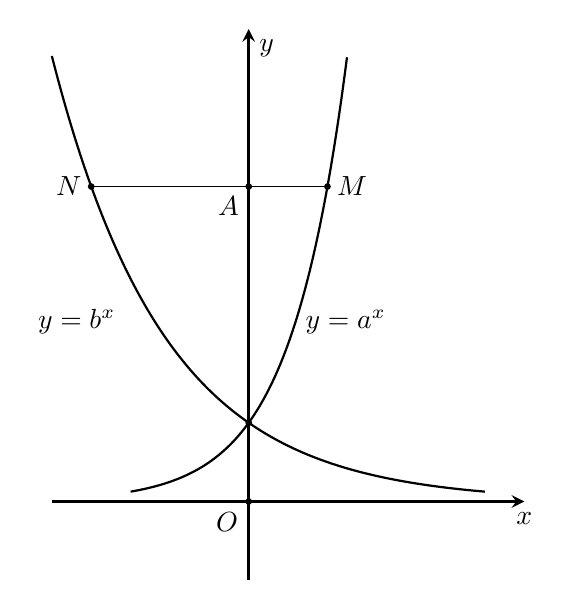
\begin{tikzpicture}[>=stealth, scale=1]
		\draw[->, line width = 1pt] (-2.5,0) -- (0,0) node[below left]{$O$} -- (3.5,0) node[below]{$x$};
		\draw[->, line width = 1pt] (0,-1) -- (0,0) -- (0,6) node[below right]{$y$};
		\draw[black] (0.6,2) node[above right]{$y=a^x$};
		\draw[black] (-2.8,2) node[above right]{$y=b^x$};
		\draw[black, samples=200, thick, domain=-1.5:1.25] plot(\x,{4^(\x)});
		\draw[black, samples=200, thick, domain=-2.5:3] plot(\x,{(1/2)^(\x)});
		\draw[fill=black]  (0,4) node[below left]{$A$} circle (1pt);
		\draw[fill=black]  (1,4) node[right]{$M$} circle (1pt);
		\draw[fill=black]  (-2,4) node[left]{$N$} circle (1pt);
		\draw[fill=black]  (0,0)  circle (1pt);
		\draw[fill=black]  (0,1)  circle (1pt);
		\draw (-2,4) -- (1,4);
		\end{tikzpicture}
	\end{center}
	\loigiai{
		Giả sử $M(1 ; a) \Rightarrow N\left(-3 ; b^{-3}\right)$. Mà M, N, A thẳng hàng suy ra $a=b^{-3} \Leftrightarrow a \cdot b^{3}=1$.}
\end{vd}
\subsubsection{Câu hỏi trắc nghiệm}	
\begin{ex}%[2D2B4-3] %Câu 1.
	Trong các hàm số dưới đây, hàm số nào nghịch biến trên tập số thực $\mathbb{R}$?
	\choice
	{$y=\left(\dfrac{\pi}{3}\right)^x$}
	{$y=\log_{\tfrac{1}{2}}x$}
	{$y=\log_{\tfrac{\pi}{4}}\left(2x^2+1\right)$}
	{\True $y=\left(\dfrac{2}{e}\right)^x$}
	\loigiai{
		Hàm số $y=\log_{\tfrac{1}{2}}x$ có TXĐ $\mathscr{D}=(0;+\infty)$ nên không thỏa mãn.\\
		Do $\dfrac{\pi}{3}>1$ nên hàm số $y=\left(\dfrac{\pi}{3}\right)^x$ đồng biến trên $\mathbb{R}$.\\
		Do $0<\dfrac{2}{e}<1$ nên hàm số $y=\left(\dfrac{2}{e}\right)^x$ nghịch biến trên $\mathbb{R}$.\\
		Hàm số $y=\log_{\tfrac{\pi}{4}}\left(2x^2+1\right)$ có $y'=\dfrac{4x}{\left(2x^2+1\right)\ln\left(\dfrac{\pi}{4}\right)}$ đổi dấu khi $x$ đi qua $0$ nên không nghịch biến trên $\mathbb{R}$.}
\end{ex}
\begin{ex}%[2D2B4-3] %Câu 2.
	Cho hai hàm số $y=f(x)=\log_ax$ và $y=g(x)=a^x$. Xét các mệnh đề sau:\\
	I. Đồ thị của hai hàm số $f(x)$ và $g(x)$ luôn cắt nhau tại một điểm.\\
	II. Hàm số $f(x)+g(x)$ đồng biến khi $a>1$, nghịch biến khi $0<a<1$.\\
	III. Đồ thị hàm số $f(x)$ nhận trục $Oy$ làm tiệm cận.\\
	IV. Chỉ có đồ thị hàm số $f(x)$ có tiệm cận.\\
	Số mệnh đề đúng là 
	\choice
	{$1$}
	{$4$}
	{\True $2$}
	{$3$}
	\loigiai{
		I. sai vì có đồ thị hàm số $y=f(x)=\log_2x$ và $y=g(x)=2^x$ đối xứng nhau qua đường thẳng $y=x$ nhưng không cắt nhau, đồ thị hàm số $y=f(x)=\log_{\sqrt{2}}x$ và $y=g(x)=\sqrt2^x$ cắt nhau tại hai điểm $A(2; 2)$ và $B(4; 4)$.\\
		II. đúng do tính chất đơn điệu của hàm số mũ và hàm số lôgarit.\\
		III. đúng do $\lim\limits_{x\to 0^+} f(x)=\lim\limits_{x\to 0^+}\log_ax=-\infty$ khi $a>1$ và $\lim\limits_{x\to 0^+} f(x)=\lim\limits_{x\to 0^+}\log_ax=+\infty$ khi $0<a<1$ nên đồ thị hàm số $f(x)$ nhận trục $Oy$ làm tiệm cận (tiệm cận đứng)\\
		IV. sai vì đồ thị hàm số $y=g(x)=a^x$ có tiệm cận ngang là đường thẳng $y=0$.}
\end{ex}
\begin{ex}%[2D2B4-3] %Câu 3.
	Điều kiện nào của $a$ cho dưới đây làm cho hàm số $f(x)=(1+\ln a)^x$ đồng biến trên $\mathbb{R}$?
	\choice
	{$\dfrac{1}{e}<a<1$}
	{\True $a>1$}
	{$a>0$}
	{$a>e$}
	\loigiai{
		Hàm số $f(x)$ đồng biến trên $\mathbb{R}$ khi $\heva{&a>0\\&1+\ln a>1}\Leftrightarrow\heva{&a>0\\&a>\mathrm{e}^{\circ}}\Rightarrow a>1$.}
\end{ex}
\begin{ex}%[2D2B4-3] %Câu 4.
	Chọn mệnh đề sai trong các mệnh đề sau
	\choice
	{Hàm số $y=\log_2(\sqrt{x}+1)$ đồng biến trên $[0;+\infty)$}
	{Hàm số $y=\log_{0,2}x$ nghịch biến trên $(0;+\infty)$}
	{Hàm số $y=\log_2x$ đồng biến trên $(0;+\infty)$}
	{\True Hàm số $y=\log_2x$ đồng biến trên $[0;+\infty)$}
	\loigiai{
		Hàm số $y=\log_2x$ có tập xác định $\mathscr{D}=(0;+\infty)$ nên không đồng biến trên $[0;+\infty)$.}
\end{ex}
\begin{ex}%[2D2Y4-3] %Câu 5.
	Hàm số nào sau đây đồng biến trên khoảng $(-\infty;+\infty)$. 
	\choice
	{$y=\left(\dfrac{\sqrt{3}+\sqrt{2}}{4}\right)^x$}
	{$y=\left(\sqrt{3}-\sqrt{2}\right)^x$}
	{$y=\left(\dfrac{2}{e}\right)^x$}
	{\True $y=\left(\dfrac{\sqrt{3}+\sqrt{2}}{3}\right)^x$}
	\loigiai{
		Hàm số mũ $y=a^x$ với cơ số $a>1$ đồng biến trên $(-\infty;+\infty)$.\\
		Do đó hàm số $y=\left(\dfrac{\sqrt{3}+\sqrt{2}}{3}\right)^x$ đồng biến trên khoảng $(-\infty;+\infty)$ vì $\dfrac{\sqrt{3}+\sqrt{2}}{3}>1$.}
\end{ex}
\begin{ex}%[2D2B4-3] %Câu 6.
	Cho hai hàm số $f(x)=\log_2x$, $g(x)=2^x$. Xét các mệnh đề sau:\\
	(I). Đồ thị hai hàm số đối xứng nhau qua đường thẳng $y=x$.\\
	(II). Tập xác định của hai hàm số trên là $\mathbb{R}$.\\
	(III). Đồ thị hai hàm số cắt nhau tại đúng $1$ điểm.\\
	(IV). Hai hàm số đều đồng biến trên tập xác định của nó.\\
	Có bao nhiêu mệnh đề đúng trong các mệnh đề trên. 
	\choice
	{\True $2$}
	{$3$}
	{$1$}
	{$4$}
	\loigiai{
		Các mệnh đề đúng là\\
		(I). Đồ thị hai hàm số đối xứng nhau qua đường thẳng $y=x$.\\
		(IV). Hai hàm số đều đồng biến trên tập xác định của nó.}
\end{ex}
\begin{ex} %[2D2B4-3] %Câu 7.
	Cho $a$, $b$, $c$ là các số thực dương khác $1$. Hình vẽ bên là đồ thị các hàm số $y=a^x, y=b^x, y=\log_cx$.\\
	\begin{center}
		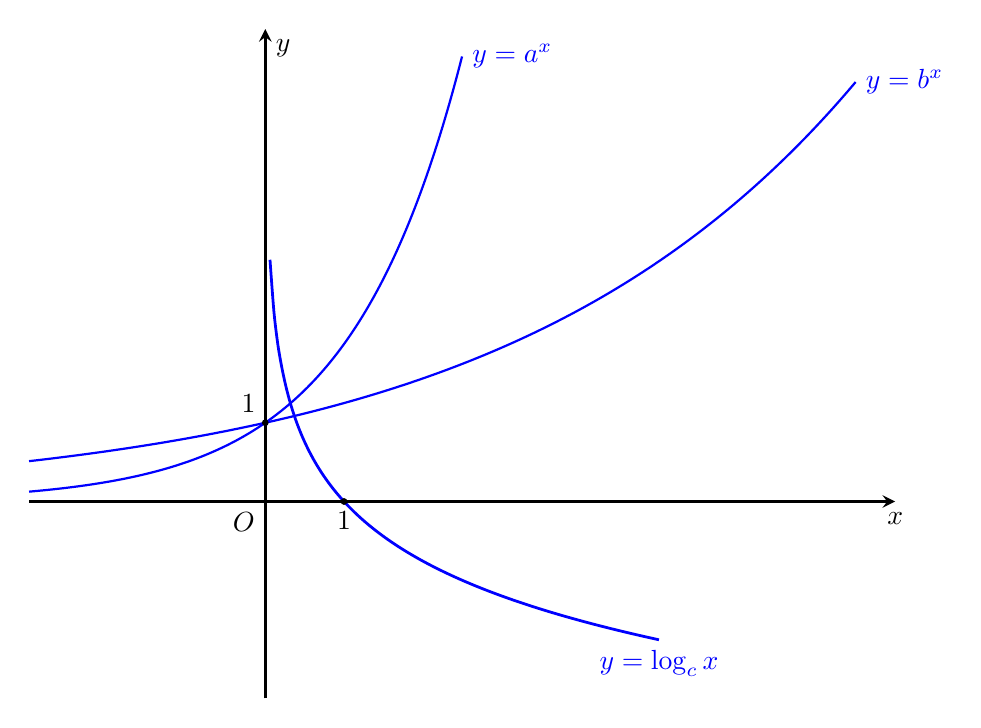
\begin{tikzpicture}[>=stealth, scale=1]
		\draw[->, line width = 1pt] (-3,0) -- (0,0) node[below left]{$O$} -- (8,0) node[below]{$x$};
		\draw[->, line width = 1pt] (0,-2.5) -- (0,0) -- (0,6) node[below right]{$y$};
		\draw[blue, samples=200, thick, domain=-3:2.5] plot(\x,{2^(\x)})node[right]{$y=a^x$};
		\draw[blue, samples=200, thick, domain=-3:7.5] plot(\x,{(1.25)^(\x)})node[right]{$y=b^x$};
		\draw[smooth, blue, line width=1,samples=100] plot[domain=0.06:5] (\x,{ln(\x)/ln(0.4)}) node[below]{$y=\log_cx$};
		\draw[fill=black]  (1,0) node[below]{$1$} circle (1pt);
		\draw[fill=black]  (0,1) node[above left]{$1$} circle (1pt);
		\end{tikzpicture}
	\end{center}
	Mệnh đề nào sau đây đúng? 
	\choice
	{$a<b<c$}
	{\True $c<b<a$}
	{$a<c<b$}
	{$c<a<b$}
	\loigiai{ 
		\begin{center}
			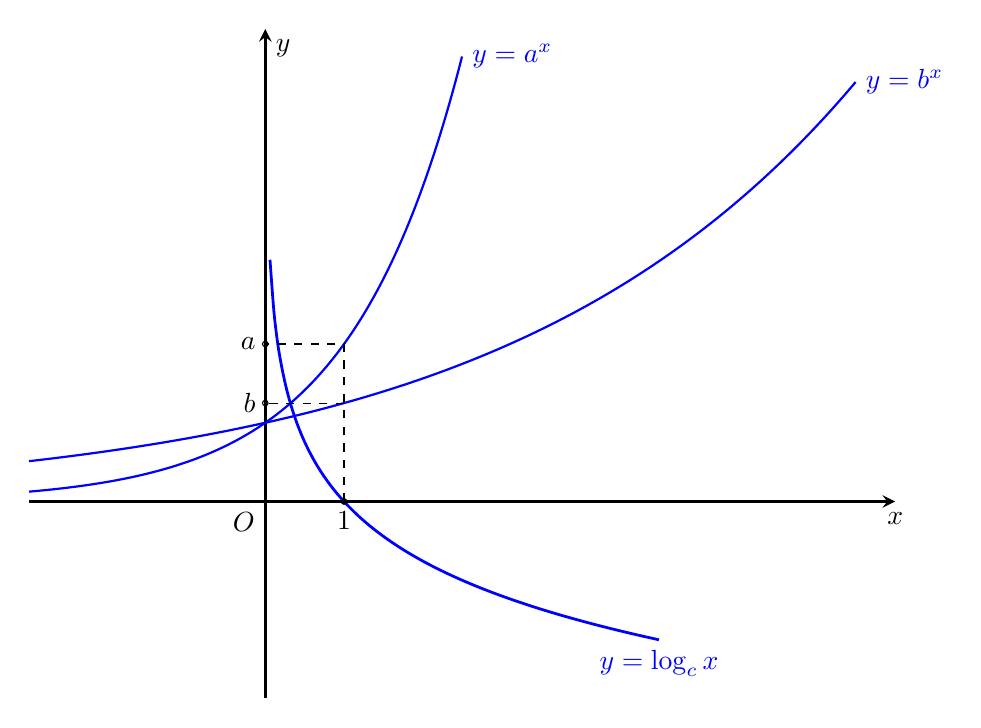
\begin{tikzpicture}[>=stealth, scale=1]
			\draw[->, line width = 1pt] (-3,0) -- (0,0) node[below left]{$O$} -- (8,0) node[below]{$x$};
			\draw[->, line width = 1pt] (0,-2.5) -- (0,0) -- (0,6) node[below right]{$y$};
			\draw[blue, samples=200, thick, domain=-3:2.5] plot(\x,{2^(\x)})node[right]{$y=a^x$};
			\draw[blue, samples=200, thick, domain=-3:7.5] plot(\x,{(1.25)^(\x)})node[right]{$y=b^x$};
			\draw[smooth, blue, line width=1,samples=100] plot[domain=0.06:5] (\x,{ln(\x)/ln(0.4)}) node[below]{$y=\log_cx$};
			\draw[fill=black]  (1,0) node[below]{$1$} circle (1pt);
			\draw  (0,2) node[ left]{$a$} circle (1pt);
			\draw  (0,1.25) node[ left]{$b$} circle (1pt);
			\draw[dashed] (1,0) -- (1,2) -- (0,2)
			(1,1.25) -- (0,1.25);
			\end{tikzpicture}
		\end{center}
		Vì hàm số $y=\log_cx$ nghịch biến nên $0<c<1$, các hàm số $y=a^x, y=b^x$ đồng biến nên $a>1; b>1$ nên $c$ là số nhỏ nhất trong ba số.\\
		Đường thẳng $x=1$ cắt hai hàm số $y=a^x, y=b^x$ tại các điểm có tung độ lần lượt là $a$ và $b$, dễ thấy $a>b$ (hình vẽ). Vậy $c<b<a$.}
\end{ex}
\begin{ex}%[2D2B4-3] %Câu 8.
	Trong các khẳng định sau, khẳng định nào đúng?
	\choice
	{\True Hàm số $y=\mathrm{e}^{10x+2017}$ đồng biến trên $\mathbb{R}$}
	{Hàm số $y=\log_{1,2}x$ nghịch biến trên khoảng $(0;+\infty)$}
	{$a^{x+y}=a^x+a^y;\forall a>0,a\neq 1,x,y\in\mathbb{R}$}
	{$\log(a+b)=\log a+\log b;\forall a>0,b>0$}
	\loigiai{
		B sai vì cơ số $1,2>1$ nên hàm số đồng biến trên TXĐ.\\
		C sai vì $a^{x+y}=a^x\cdot a^y;\forall a>0,a\neq 1,x,y\in\mathbb{R}$.\\
		D sai vì $\log(ab)=\log a+\log b;\forall a>0,b>0$.}
\end{ex}
\begin{ex}%[2D2K4-3] %Câu 9.
	Biết hàm số $y=f(x)$ có đồ thị đối xứng với đồ thị hàm số $y=3^x$ qua đường thẳng $x=-1$.\\
	\begin{center}
		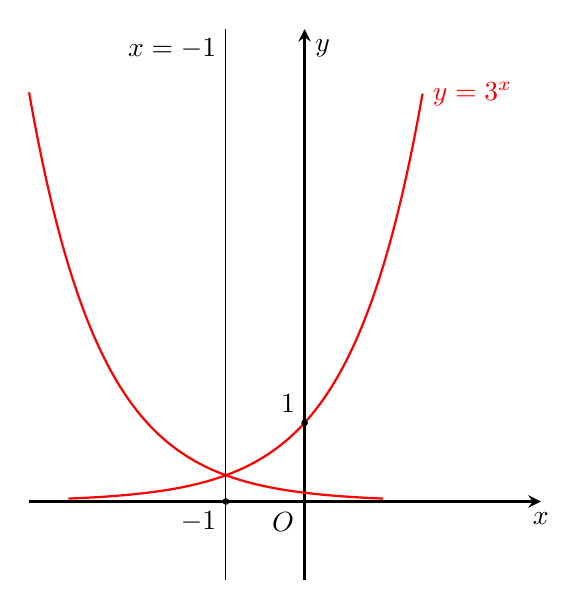
\begin{tikzpicture}[>=stealth, scale=1]
		\draw[->, line width = 1pt] (-3.5,0) -- (0,0) node[below left]{$O$} -- (3,0) node[below]{$x$};
		\draw[->, line width = 1pt] (0,-1) -- (0,0) -- (0,6) node[below right]{$y$};
		\draw[red, samples=200, thick, domain=-3:1.5] plot(\x,{3^(\x)})node[right]{$y=3^x$};
		\draw[red, samples=200, thick, domain=-3.5:1] plot(\x,{(1/3)^(\x+1)/3});
		\draw  (-1,0) node[ below left]{$-1$} circle (1pt);
		\draw (-1,-1) -- (-1,6);
		\draw[black] (-1,5.5) node[above left]{$x=-1$};
		\draw[fill=black]  (0,1) node[above left]{$1$} circle (1pt);
		\end{tikzpicture}
	\end{center}
	Chọn khẳng định đúng trong các khẳng định sau: 
	\choice
	{$f(x)=\dfrac{1}{{3\cdot 3}^x}$}
	{\True $f(x)=\dfrac{1}{{9\cdot 3}^x}$}
	{$f(x)=\dfrac{1}{3^x}-\dfrac{1}{2}$}
	{$f(x)=-2+\dfrac{1}{3^x}$}
	\loigiai{
		Trên đồ thị hàm số $y=3^x$ lấy $M(x_0; y_0)$ và gọi $N\left(x; f(x)\right)$ là điểm thuộc đồ thị hàm số $f(x)$ và đối xứng với $M$ qua đường thẳng $x=-1$.\\
		Khi đó $\heva{&\dfrac{x+x_0}{2}=-1\\&f(x)-y_0=0}\Leftrightarrow\heva{&x_0=-x-2\\&y_0=f(x).}$ \\
		Thay vào hàm số ban đầu ta được: $f(x)=3^{-x-2}=\dfrac{1}{{9\cdot 3}^x}$.}
\end{ex}
\begin{ex}%[2D2B4-3] %Câu 10.
	Chọn câu khẳng định đúng trong các câu sau: 
	\choice
	{Hàm số $y=a^x$ đồng biến khi $0<a<1$}
	{Đồ thị hàm số $y=a^x$ luôn nằm bên phải trục tung}
	{\True Đồ thị hàm số $y=a^x$ và $y=\left(\dfrac{1}{a}\right)^x$ đối xứng nhau qua trục tung, với $a>0;a\neq 1$}
	{Đồ thị hàm số $y=a^x$ và $y=\left(\dfrac{1}{a}\right)^x$ đối xứng nhau qua trục hoành, với $a>0;a\neq 1$}
	\loigiai{
		Cách 1.\\
		* Hàm số $y=a^x$ đồng biến khi $a>1$ và nghịch biến khi $0<a<1$ nên A sai.\\
		* Hàm số $y=a^x$ có tập xác định là $\mathbb{R}$ nên B sai.\\
		* Đồ thị của hai hàm số $y=a^x$ và $y=\left(\dfrac{1}{a}\right)^x$ đều nằm trên trục hoành suy ra không thể đối xứng nhau qua trục hoành nên D sai.\\
		* Vậy đáp án đúng là C.\\
		Cách 2.
		Ta có $a^{-x}=\dfrac{1}{a^x}=\left(\dfrac{1}{a}\right)^x$, với $a>0;a\neq 1$. Suy ra đồ thị hàm số $y=a^x$ và $y=\left(\dfrac{1}{a}\right)^x$ đối xứng nhau qua trục tung.}
\end{ex}
\begin{ex}%[2D2K4-3] %Câu 11.
	Tìm tất cả các giá trị thực của tham số $m$ để hàm số $y=\dfrac{m\ln x-2}{\ln x-m-1}$ nghịch biến trên $\left(\mathrm{e}^2;+\infty\right)$. 
	\choice
	{$m\leq-2$ hoặc $m=1$}
	{$m <-2$ hoặc $m=1$}
	{\True $m <-2$}
	{$m <-2$ hoặc $m>1$}
	\loigiai{
		Tập xác định $\mathscr{D}=(0;+\infty)\setminus\left\{\mathrm{e}^{m+1}\right\}$.\\
		Cách 1: $y'=\dfrac{-m^2-m+2}{x(\ln x-m-1)^2}$.\\
		Vậy yêu cầu bài toán tương đương $\heva{&-m^2-m+2<0\\&\mathrm{e}^{m+1}\notin\left(\mathrm{e}^2;+\infty\right)}\Leftrightarrow\heva{&\hoac{&m>1\\&m <-2}\\&m+1\leq 2}\Leftrightarrow m <-2$.\\
		Cách 2: Đặt $t=\ln x$, ta biết rằng hàm số $f(x)=\ln x$ đồng biến trên $\left(\mathrm{e}^2;+\infty\right)$.\\
		Xét hàm số $g(t)=\dfrac{mt-2}{t-m-1}$ với $t\in(2;+\infty)$, ta có $g'(t)=\dfrac{-m^2-m+2}{(t-m-1)^2}$.\\
		Vậy hàm số ban đầu nghịch biến trên $\left(\mathrm{e}^2;+\infty\right)\Leftrightarrow$ hàm số $g$ nghịch biến trên $(2;+\infty)$ \\
		$ \Leftrightarrow\heva{&g'(t)<0\\&m+1\notin(2;+\infty)}\Leftrightarrow\heva{&-m^2-m+2<0\\&m+1\leq 2}\Leftrightarrow\heva{&\hoac{&m>1\\&m <-2}\\&m+1\leq 2}\Leftrightarrow\heva{&\hoac{&m>1\\&m <-2}\\&m\leq 1}\Leftrightarrow m <-2 $.}
\end{ex}
\begin{ex}%[2D2B4-3] %Câu 12.
	Cho $a$, $b$, $c$ dương và khác $1$. Đồ thị các hàm số $y=\log_ax$, $y=\log_bx$, $y=\log_cx$ như hình vẽ.\\
	\begin{center}
		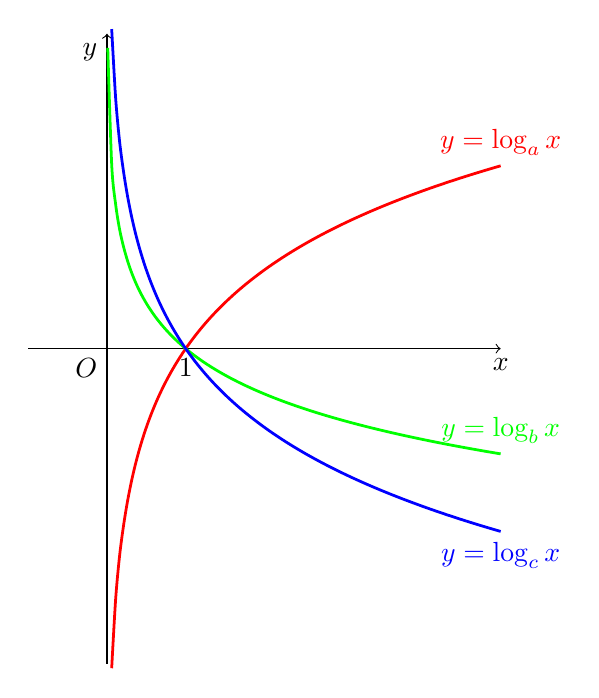
\begin{tikzpicture}
		\draw[->] (-1,0)--(0,0) node[below left]{$O$}--(5,0) node[below]{$x$};
		\draw[->] (0,-4)--(0,4) node[below left]{$y$};
		\draw[smooth, red, line width=1,samples=100] plot[domain=0.06:5] (\x,{log2(\x)}) node[above]{$y=\log_ax$};
		\draw[smooth, green, line width=1,samples=100] plot[domain=0.01:5] (\x,{ln(\x)/ln(0.3)}) node[above]{$y=\log_bx$};
		\draw[smooth, blue, line width=1,samples=100] plot[domain=0.06:5] (\x,{ln(\x)/ln(0.5)}) node[below]{$y=\log_cx$};
		\draw[dashed] (1,0) node[below]{$1$};
		\end{tikzpicture}
	\end{center}
	Khẳng định nào dưới đây đúng?
	\choice
	{\True $a>c>b$}
	{$a>b>c$}
	{$c>b>a$}
	{$b>c>a$}
	\loigiai{
		Dựa vào đồ thị ta thấy đồ thị hàm số $y=\log_ax$ đồng biến trên tập xác định nên $a>1$.\\
		Đồ thị hàm số $y=\log_bx$ và $y=\log_cx$ nghịch biến trên tập xác định nên $0<b<1$, $0<c<1$.\\
		Suy ra $a>b$ và $a>c$.\\
		Mặt khác với $x>1$ ta có $\log_bx>\log_cx\Rightarrow b<c$. Vậy $a>c>b$.}
\end{ex}
\begin{ex}%[2D2K4-3] %Câu 13.
	Cho hai đường cong $(C_1)$: $y=3^x\left(3^x-m+2\right)+m^2-3m$ và $(C_2)$: $y=3^x+1$. Để $(C_1)$ và $(C_2)$ tiếp xúc nhau thì giá trị của tham số $m$ bằng
	\choice
	{$m=\dfrac{5-2\sqrt{10}}{3}$}
	{$m=\dfrac{5+3\sqrt{2}}{3}$}
	{\True $m=\dfrac{5+2\sqrt{10}}{3}$}
	{$m=\dfrac{5-3\sqrt{2}}{3}$}
	\loigiai{
		Đặt $t=3^x (t>0)$ suy ra $(C_1)$: $y=3^x\left(3^x-m+2\right)+m^2-3m=t^2+(2-m)t+m^2-3m$.\\
		và $(C_2)$: $y=3^x+1=t+1$.\\
		Để $(C_1)$ và $(C_2)$ tiếp xúc nhau thì hệ $\heva{&t^2+(2-m)t+m^2-3m=t+1\\&2t+2-m=1}$ có nghiệm $t>0$.\\
		$\heva{&t^2+(2-m)t+m^2-3m=t+1\\&2t+2-m=1}\Leftrightarrow\heva{&m=2t+1\\&3t^2-2t-3=0}\Leftrightarrow\heva{&m=2t+1\\&t=\dfrac{1\pm\sqrt{10}}{3}.}$ \\
		Do nghiệm $t>0$ nên $t=\dfrac{1+\sqrt{10}}{3}\Rightarrow m=\dfrac{5+2\sqrt{10}}{3}$.}
\end{ex}
\begin{ex}%[2D2K4-3] %Câu 14.
	Hàm số nào sau đây đồng biến trên từng khoảng xác định của nó?
	\choice
	{$y=(\sqrt{2}-1)^x$}
	{$y=\log_2\left(x^2+1\right)$}
	{\True $y=\dfrac{1}{3}x^3-x^2+x-3$}
	{$y=x^4-2x^2+1$}
	\loigiai{
		• Xét hàm số $y=(\sqrt{2}-1)^x$ có cơ số $a=\sqrt{2}-1\in(0;1)$ nên hàm số luôn nghịch biến trên từng khoảng xác định của nó. Vậy $y=(\sqrt{2}-1)^x$ sai.\\
		• Xét hàm số $y=\log_2\left(x^2+1\right)$. Tập xác định $\mathscr{D}=\mathbb{R}$.\\
		$y'=\dfrac{2x}{\left(x^2+1\right)\ln 2}$ không mang dấu dương tren tờn miền xác định nên không thể đồng biến trên từng khoảng xác định của nó. Vậy $y=\log_2\left(x^2+1\right)$ sai.\\
		• Xét hàm số $y=x^4-2x^2+1$ có $y'=4x\left(x^2-1\right)>0\Leftrightarrow\hoac{&-1<x<0\\&x>1}$ nên hàm số không đồng biến trên từng khoảng xác định của nó. Vậy $y=x^4-2x^2+1$ sai.\\
		• Xét hàm số $y=\dfrac{1}{3}x^3-x^2+x-3$.\\
		$y'=x^2-2x+1=(x-1)^2\geq 0$ (Dấu $''=‘‘$ xảy ra tại $x=1$).\\
		Suy ra hàm số đồng biến trên khoảng $(-\infty;+\infty)$.}
\end{ex}


\Closesolutionfile{ans}
% \DAPAN
% \inputansbox{10}{ans/ans-2D2-4(2)}
%\begin{indapan}
%	{10}{ans/ansCD2D2-4}
%\end{indapan}
%\begin{indapan}
%	{10}{ans/ansCD2D2-4}
%\end{indapan}
\Opensolutionfile{ans}[ans/ans-2D2-4(3)]

\begin{dang}{Sự biến thiên và đồ thị của hàm số mũ – hàm số logarit}
\end{dang}
\begin{ex}%[Dự án TLDH2-Nhóm Latex, Kiều Ngân]%[2D2K4-3]%Câu 15.
	Tìm tập hợp tất cả các giá trị của tham số thực $m$ để hàm số $y=\ln\left(x^2+1\right)-mx+1$ đồng biến trên khoảng $(-\infty;+\infty)$. 
	\choice
	{$(-\infty;-1)$}
	{$(-1;1)$}
	{$[-1;1]$}
	{\True $(-\infty;-1]$}
	\loigiai{		
		Tập xác định $\mathscr{D}=\mathbb{R}$. Ta có $y'=\dfrac{2x}{x^2+1}-m$.\\
		Hàm số đồng biến trên khoảng $(-\infty;+\infty)$ khi và chỉ khi
		$$y'=\dfrac{2x}{x^2+1}-m\geq 0,\forall x\in\mathbb{R}\Leftrightarrow\dfrac{2x}{x^2+1}\geq m,\forall x\in\mathbb{R}.$$
		Xét hàm số $y=\dfrac{2x}{x^2+1}$ ta có $y'=\dfrac{-2x^2+2}{\left(x^2+1\right)^2}$; $y'=0\Leftrightarrow x=\pm 1$.\\
		Bảng biến thiên:
		\begin{center}
			
\begin{tikzpicture}[>=stealth]
			\tkzTabInit[nocadre=false,lgt=1.2,espcl=2,deltacl=0.5]
			{$x$/.7 ,$y'$/.7,$y$/1.5}
			{$-\infty$, $-1$, $1$, $+\infty$}
			\tkzTabLine{,-,$0$,+,$0$,-,}
			\tkzTabVar{+/$0$,-/$-1$,+/$1$,-/$0$}
			\end{tikzpicture}
		\end{center}
		Dựa vào bảng biến thiên ta thấy $m\leq-1$ thỏa điều kiện đề bài.}
\end{ex}
\begin{ex}%[Dự án TLDH2-Nhóm Latex, Kiều Ngân]%[2D2K4-3]%Câu 16.
	Gọi $S$ là tập các giá trị của tham số thực $m$ để hàm số $y=x^2+\ln(x+m+2)$ đồng biến trên tập xác định của nó. Biết $S=\left(-\infty;a+\sqrt{b}\right]$. Tính tổng $K=a+b$.
	\choice
	{$K=-5$}
	{$K=5$}
	{\True $K=0$}
	{$K=2$}
	\loigiai{
		Điều kiện xác định: $x >-m-2$.\\
		Ta có $y’=2x+\dfrac{1}{x+m+2} =\dfrac{2x^2+2(m+2)x+1}{x+m+2}$, $y’=0\Leftrightarrow 2x^2+2(m+2)x+1=0$.
		\begin{itemize}
			\item TH1: $\Delta’=m^2+4m+2\leq 0\Leftrightarrow-2-\sqrt{2}\leq m\leq-2+\sqrt{2}$, khi đó $y’\geq 0,\,\forall x\in (-m-2;+\infty)$.
			\item $\Delta’>0\Leftrightarrow\hoac{&m <-2-\sqrt{2}\\&m >-2+\sqrt{2}}$, khi đó $y’=0$ có hai nghiệm phân biệt
			$$x_1=\dfrac{-(m+2)-\sqrt{m^2+4m+2}}{2},\, x_2=\dfrac{-(m+2)+\sqrt{m^2+4m+2}}{2}.$$
			Bảng biến thiên:
			\begin{center}
				
\begin{tikzpicture}[>=stealth]
				\tkzTabInit[nocadre=false,lgt=1.2,espcl=2,deltacl=0.5]
				{$x$/.7 ,$y'$/.7,$y$/1.5}
				{$-\infty$, $x_1$, $x_2$, $+\infty$}
				\tkzTabLine{,+,$0$,-,$0$,+,}
				\tkzTabVar{-/$-\infty$,+/,-/,+/$+\infty$}
				\end{tikzpicture}
			\end{center}
			\allowdisplaybreaks
			\begin{eqnarray*}
				y’\geq 0,\,\forall x\in (-m-2;+\infty)&\Leftrightarrow& x_2\leq-m-2\Leftrightarrow\dfrac{-(m+2)+\sqrt{m^2+4m+2}}{2}\leq-m-2\\
				&\Leftrightarrow&\sqrt{m^2+4m+2}\leq-m-2\Leftrightarrow\heva{&m^2+4m+2\leq m^2+4m+4\\&m\leq-2\\&m^2+4m+2\geq 0}\\
				&\Leftrightarrow&\heva{&m\leq-2\\&\hoac{&m\leq-2-\sqrt{2}\\&m\geq-2+\sqrt{2}}}\Leftrightarrow m\leq-2-\sqrt{2}.
			\end{eqnarray*}
		\end{itemize}
		Kết hợp 2 trường hợp ta được $S=(-\infty;-2+\sqrt{2}]\Rightarrow a=-2$, $b=2$ nên $K=a+b=0$.}
\end{ex}
\begin{ex}%[Dự án TLDH2-Nhóm Latex, Kiều Ngân]%[2D2K4-3]%Câu 17.
	\immini{
		Cho các hàm số $y=\log_ax$ và $y=\log_bx$ có đồ thị như hình vẽ bên. Đường thẳng $x=5$ cắt trục hoành, đồ thị hàm số $y=\log_ax$ và $y=\log_bx$ lần lượt tại $A$, $B$ và $C$. Biết rằng $CB=2AB$. Mệnh đề nào sau đây là đúng?
		\choice
		{$a=b^2$}
		{$a^3=b$}
		{\True $a=b^3$}
		{$a=5b$}
	}{
		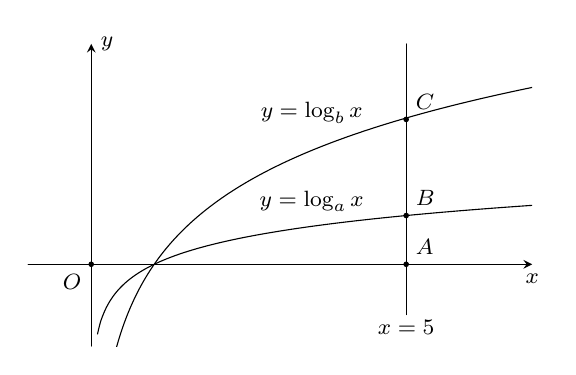
\begin{tikzpicture}[>=stealth,line join=round,line cap=round,font=\footnotesize,scale=0.8]
		\draw[->] (-1,0)--(7,0)node[below]{$x$};
		\draw[->] (0,-1.3)--(0,3.5)node[right]{$y$};
		\clip (-1,-1.3)rectangle (7,3.5);		
		\draw[smooth,samples=300]
		plot[domain=0.1:7](\x,{ln(\x)/ln 2});
		\draw[smooth,samples=300]
		plot[domain=0.1:7](\x,{ln(\x)/ln 8});
		\draw (5,-0.8)--(5,3.5);
		\draw (5,-1) node {$x=5$};
		\draw (3.5,1) node {$y=\log_a x$};
		\draw (3.5,2.4) node {$y=\log_b x$};
		\draw[fill=black] (0,0) circle (1pt) node[below left]{$O$};
		\draw[fill=black] (5,0) circle (1pt) node[above right]{$A$};
		\draw[fill=black] (5,0.774) circle (1pt) node[above right]{$B$};
		\draw[fill=black] (5,2.3) circle (1pt) node[above right]{$C$};
		\end{tikzpicture}
	}
	\loigiai{		
		Theo giả thiết, ta có $A(5;0)$, $B(5;\log_a5)$, $C(5;\log_b5)$.\\
		Ta có
		\begin{eqnarray*}
			CB=2AB&\Rightarrow&\overrightarrow{CB}=2\overrightarrow{BA}\\
			&\Rightarrow&\log_a5-\log_b5=2\cdot(-\log_a5) \\
			&\Leftrightarrow& 3\log_a5=\log_b5\Leftrightarrow\log_a5=\dfrac{1}{3}\log_b5\\
			&\Leftrightarrow&\log_a5=\log_{b^3}5\Leftrightarrow a=b^3.
		\end{eqnarray*}
	}
\end{ex}
\begin{ex}%[Dự án TLDH2-Nhóm Latex, Kiều Ngân]%[2D2K4-3]%Câu 18.
	Cho hàm số $y=-\log_2x$ có đồ thị $(C)$. Hàm số nào sau đây có đồ thị đối xứng với $(C)$ qua đường thẳng $y=x$?
	\choice
	{$y=2^x$}
	{$y=2^{\tfrac{1}{x}}$}
	{\True $y=2^{-x}$}
	{$y=2^{\tfrac{x}{2}}$}
	\loigiai{		
		Trước tiên ta đưa hàm số về dạng chuẩn $y=-\log_2x=\log_{\tfrac{1}{2}}x$.\\
		Suy ra hàm số cần tìm là $y=\left(\dfrac{1}{2}\right)^x=2^{-x}$.}
\end{ex}
\begin{ex}%[Dự án TLDH2-Nhóm Latex, Kiều Ngân]%[2D2K4-3]%Câu 19.
	\immini{
		Biết hai hàm số $y=a^x$ và $y=f(x)$ có đồ thị như hình vẽ đồng thời đồ thị của hai hàm số này đối xứng nhau qua đường thẳng $d\colon y=-x$. Tính $f\left(-a^3\right)$.
		\choice
		{$f\left(-a^3\right)=-a^{-3a}$}
		{$f\left(-a^3\right)=-\dfrac{1}{3}$}
		{\True $f\left(-a^3\right)=-3$}
		{$f\left(-a^3\right)=-a^{3a}$}
	}{
		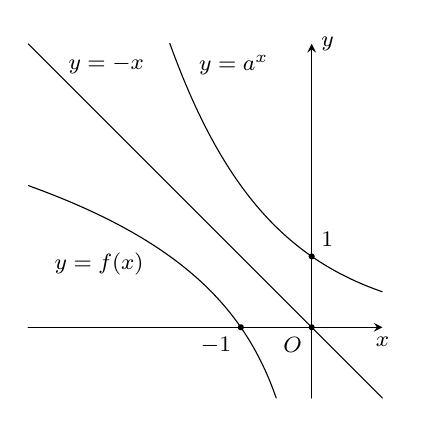
\begin{tikzpicture}[>=stealth,line join=round,line cap=round,font=\footnotesize,scale=0.9]
		\draw[->] (-4,0)--(1,0)node[below]{$x$};
		\draw[->] (0,-1)--(0,4)node[right]{$y$};
		\clip (-4,-1)rectangle (1,4);		
		\draw[smooth,samples=300]
		plot[domain=-4:1](\x,{0.5^(\x)});
		\draw[smooth,samples=300]
		plot[domain=-4:-0.5](\x,{ln(-\x)/ln 2});
		\draw (1,-1)--(-4,4);
		\draw (-2.9,3.7) node {$y=-x$};
		\draw (-1.1,3.7) node {$y=a^x$};
		\draw (-3,0.9) node {$y=f(x)$};
		\draw[fill=black] (0,0) circle (1pt) node[below left]{$O$};
		\draw[fill=black] (-1,0) circle (1pt) node[below left]{$-1$};
		\draw[fill=black] (0,1) circle (1pt) node[above right]{$1$};
		\end{tikzpicture}
	}
	\loigiai{		
		Giả sử $M(x_M;y_M)$ là điểm thuộc hàm số $y=a^x$; $N(x_0;y_0)$ là điểm đối xứng của $M$ qua đường thẳng $y=-x$.\\
		Gọi $I$ là trung điểm của $MN\Rightarrow I\left(\dfrac{x_M+x_0}{2};\dfrac{y_M+y_0}{2}\right)$.\\
		Vì $M$, $N$ đối xứng nhau qua $d\Rightarrow\heva{&I\in d\\&\overrightarrow{MN}\parallel{\overrightarrow{n}}_d}\Leftrightarrow\heva{&\dfrac{y_M+y_0}{2}=-\dfrac{x_M+x_0}{2}\\&\dfrac{x_M-x_0}{1}=\dfrac{y_M-y_0}{1}}\Leftrightarrow\heva{&x_0=-y_M\\&y_0=-x_M}$.\\
		Ta có $M\left(x_M;y_M\right)$ thuộc đồ thị hàm số $y=a^x$ nên $y_M=a^{x_M}$.\\
		Do đó $x_0=-y_{M}=-a^{x_M}=-a^{-y_0}\Rightarrow-y_0=\log_a(-x_0)\Leftrightarrow y_0=-\log_a(-x_0)$. Điều này chứng tỏ điểm $N$ thuộc đồ thị hàm số $f(x)=-\log_a(-x)$.\\
		Khi đó $f\left(-a^3\right)=-\log_aa^3=-3$.}
\end{ex}
\begin{ex}%[Dự án TLDH2-Nhóm Latex, Kiều Ngân]%[2D2K4-3]%Câu 20.
	Trong mặt phẳng với hệ tọa độ $Oxy$, cho hình vuông $ABCD$ có diện tích bằng $36$. Đường thẳng chứa cạnh $AB$ song song với trục $Ox$; các đỉnh $A$, $B$ và $C$ lần lượt nằm trên đồ thị của các hàm số $y=\log_ax$, $y=\log_{\sqrt{a}}x$ và $y=\log_{\sqrt[3]{a}}x$ với $a$ là số thực lớn hơn $1$. Tìm $a$. 
	\choice
	{$a=\sqrt{3}$}
	{$a=\sqrt[3]{6}$}
	{$a=\sqrt{6}$}
	{\True $a=\sqrt[6]{3}$}
	\loigiai{
		Do $A$, $B$ nằm trên đường thẳng $y=m$ $(m\neq 0)$.\\
		Lại có $A$, $B$ lần lượt nằm trên đồ thị của các hàm số $y=\log_ax,y=\log_{\sqrt{a}}x$.\\
		Từ đó suy ra $A\left(a^m;m\right)$, $B\left(a^{\tfrac{m}{2}};m\right)$.\\
		Vì $ABCD$ là hình vuông nên suy ra $x_c=x_B=a^{\tfrac{m}{2}}$.\\
		Lại có $C$ nằm trên đồ thị hàm số $y=\log_{\sqrt[3]{a}}x$, suy ra $C\left(a^{\tfrac{m}{2}};\dfrac{3m}{2}\right)$.\\
		Theo đề bài $S_{ABCD}=36\Rightarrow\heva{&AB=6\\&BC=6}\Rightarrow\heva{&\left|a^m-a^{\tfrac{m}{2}}\right|=6\\&\left|\dfrac{3m}{2}-m\right|=6}$
		$\Leftrightarrow\heva{&m=-12\\&a=\sqrt[6]{\dfrac{1}{3}}<1\text{ (loại)}}$ hoặc $\heva{&m=12\\&a=\sqrt[6]{3}}.$}
\end{ex}
\begin{dang}{Bài toán thực tế}
\end{dang}
\subsubsection{Các ví dụ}
\begin{vd}%[Dự án TLDH2-Nhóm Latex, Kiều Ngân]%[2D2B4-5]%Ví dụ 1.
	Một người gửi tiết kiệm số tiền $100.000.000$ đồng vào ngân hàng với lãi suất $8$\%/năm và lãi hàng năm được nhập vào vốn. Hỏi sau $15$ năm số tiền người ấy nhận về là bao nhiêu? (làm tròn đến đơn vị nghìn đồng?
	\loigiai{
		Gởi vào ngân hàng số tiền là $A$ đồng, với lãi suất hàng tháng là $r$ trên một kì hạn. Sau $n$ kì hạn, số tiền cả vốn lẫn lãi là $T=A(1+r)^n$ (kì hạn có thể là $1$ năm; $1$ tháng hoặc $k$ tháng).\\
		Theo công thức ở bài toán trên, ta có $T=100.000.000(1+8\%)^{15}=317216911{,}4$.}
\end{vd}
\begin{vd}%[Dự án TLDH2-Nhóm Latex, Kiều Ngân]%[2D2B5-6]%Ví dụ 2.
	Một người vay ngân hàng $100$ triệu đồng với lãi suất là $0,7$\%/tháng. Theo thỏa thuận cứ mỗi tháng người đó sẽ trả cho ngân hàng $5$ triệu đồng và cứ trả hàng tháng như thế cho đến khi hết nợ (tháng cuối cùng có thể trả dưới $5$ triệu). Hỏi sau bao nhiêu tháng thì người đó trả được hết nợ ngân hàng?
	\loigiai{
		\textbf{(Vay tra góp)} Một người vay vốn $A$ đồng, lãi suất $r$ trên tháng, hàng tháng trả $a$ đồng (trả cuối tháng). Số tiền nợ còn lại sau $n$ tháng là $T=A(1+r)^n-\dfrac{a}{r}[(1+r)^n-1]$.\\
		Theo công thức ở bài toán trên, ta có
		$T=100(1+0{,}7\%)^n-\dfrac{5}{0{,}7\%}[(1+0{,}7\%)^n-1]$.\\
		Sau tháng thứ $n$ trả hết nợ nên
		\begin{eqnarray*}
			&&T=100(1+0{,}7\%)^n-\dfrac{5}{0{,}7\%}[(1+0{,}7\%)^n-1]=0 \\
			&\Leftrightarrow& 
			\left(100-\dfrac{5}{0{,}7\%}\right)(1+0{,}7\%)^n=\dfrac{5}{0{,}7\%}\\
			&\Leftrightarrow& n=\log_{1+0{,}7\%}\left[-\dfrac{5}{0{,}7\%}:\left(100-\dfrac{5}{0{,}7\%}\right)\right]\\
			&\Leftrightarrow& n\approx 21{,}6.
		\end{eqnarray*}
		Vậy sau tháng thứ $22$ thì người đó trả hết nợ.}
\end{vd}
\begin{vd}%[Dự án TLDH2-Nhóm Latex, Kiều Ngân]%[2D2B5-6]%Ví dụ 3.
	Cường độ một trận động đất $M$ (richter) được cho bởi công thức $M = \log A -\log A_0$, với $A$ là biên độ rung chấn tối đa và $A_0$ là một biên độ chuẩn (hằng số). Đầu thế kỷ $20$, một trận động đất ở San Francisco có cường độ $8{,}3$ độ Richter. Trong cùng năm đó, trận động đất khác Nam Mỹ có biên độ mạnh hơn gấp $4$ lần. Cường độ của trận động đất ở Nam Mỹ là bao nhiêu?
	\loigiai{
		Cường độ trận động đất ở San Francisco là $8{,}3=\log A-\log A_0$.\\
		Trận động đất khác Nam Mỹ có biên độ là $4A$.\\
		Suy ra cường độ là $M=\log (4A)-\log A_0=\log 4+\log A-\log A_0=\log 4+8{,}3 \approx 8{,}9$.}
\end{vd}
\begin{vd}%[Dự án TLDH2-Nhóm Latex, Kiều Ngân]%[2D2K5-6]%Ví dụ 4.
	Thầy Đông gửi $5$ triệu đồng vào ngân hàng với lãi suất $0,7\%$/tháng. Chưa đầy một năm thì lãi suất tăng lên thành $1{,}15\%$/tháng. Tiếp theo, sáu tháng sau lãi suất chỉ còn $0{,}9\%$ /tháng. Thầy Đông tiếp tục gửi thêm một số tháng nữa rồi rút cả vỗn lẫn lãi được $5787710{,}707$ đồng. Hỏi thầy Đông đã gửi tổng thời gian bao nhiêu tháng?
	\loigiai{
		Gọi $a$ là số tháng mà thầy Đông gởi tiền với lãi suất $0{,}7$\%.\\
		Gọi $b$ là số tháng mà thầy Đông gởi tiền với lãi suất $0{,}9$\%.\\
		Theo đề bài, ta có phương trình
		\begin{eqnarray*}
			&&5000000(1+0{,}7\%)^a\cdot (1+1{,}15\%)^6\cdot (1+0{,}9\%)^b=5787710{,}707\quad (*) \\
			&\Leftrightarrow& (1+0{,}7\%)^a\cdot (1+0{,}9\%)^b=1{,}080790424 \\
			&\Rightarrow& \heva{&0<a<\log_{1{,}007}1{,}080790424\\&0<b<\log_{1{,}009}1{,}080790424\\&a,b\in \mathbb{N}} \\
			&\Rightarrow& \log_{1{,}009}1{,}080790424<a+b<\log_{1{,}007}1{,}080790424\\
			&\Rightarrow& 9\leq a+b\leq 11.
		\end{eqnarray*}
		Với $a+b=9$, thử $a,\,b\in \mathbb{N}$ ta thấy $(*)$ không thoả mãn.\\
		Với $a+b=10$, thử $a,\,b\in \mathbb{N}$ ta được $a=6$; $b=4$ thoả mãn $(*)$.\\
		Với $a+b=11$, thử $a,\,b\in \mathbb{N}$ ta thấy $(*)$ không thoả mãn.\\
		Vậy thầy Đông gởi tổng thời gian là $16$ tháng.}
\end{vd}
\begin{vd}%[Dự án TLDH2-Nhóm Latex, Kiều Ngân]%[2D2B5-6]%Ví dụ 5.
	Một người gởi vào ngân hàng $9{,}8$ triệu đồng theo thể thức lãi kép với lãi suất $8{,}4\%$ một năm. Hỏi theo cách đó thì sau bao nhiêu năm người đó nhận được số tiền cả vốn lẫn lãi là $20$ triệu đồng, biết rằng trong suốt quá trình gởi lãi suất không thay đổi?
	\loigiai{
		Gọi $n$ là số tháng cần tìm.\\
		Theo công thức lãi kép, ta có $20\cdot 10^6=9{,}8\cdot 10^6(1+8{,}4\%)^n\Leftrightarrow(1+8{,}4\%)^n=\dfrac{100}{49}\Leftrightarrow n\approx 8{,}84$.}
\end{vd}
\subsubsection{Câu hỏi trắc nghiệm}
\begin{ex}%[Dự án TLDH2-Nhóm Latex, Kiều Ngân]%[2D2B5-6]%Câu 1.
	Một người gửi $15$ triệu đồng vào ngân hàng theo thể thức lãi kép kỳ hạn một quý với lãi suất $1{,}65\%$ một quý. Hỏi sau bao lâu người đó có được ít nhất $20$ triệu đồng (cả vốn lẫn lãi) từ số vốn ban đầu? (Giả sử lãi suất không thay đổi)
	\choice
	{$4$ năm $1$ quý}
	{\True $4$ năm $2$ quý}
	{$4$ năm $3$ quý}
	{$5$ năm}
	\loigiai{
		Số tiền của người ấy sau $n$ kỳ hạn là $T=15\left(1+\dfrac{1{,}65}{100}\right)^n$.\\
		Theo đề bài, ta có $15\left(1+\dfrac{1{,}65}{100}\right)^n\ge 20\Leftrightarrow n\ge\log_{1+\tfrac{1{,}65}{100}}\dfrac{4}{3}\approx 17{,}58$.\\
		Vậy người đó có ít nhất $18$ quý hay $4$ năm $2$ quý để thỏa yêu cầu bài toán.}
\end{ex}
\begin{ex}%[Dự án TLDH2-Nhóm Latex, Kiều Ngân]%[2D2B5-6]%Câu 2.
	Ngày $1/7/2016$, dân số Việt Nam khoảng $91{,}7$ triệu người. Nếu tỉ lệ tăng dân số Việt Nam hàng năm là $1{,}2$\% và tỉ lệ này ổn định trong $10$ năm liên tiếp thì ngày $1/7/2026$ dân số Việt Nam khoảng bao nhiêu triệu người?
	\choice
	{$106{,}4$ triệu người}
	{$104{,}4$ triệu người}
	{$105{,}4$ triệu người}
	{\True $103{,}4$ triệu người}
	\loigiai{
		Ngày $1/7/2026$ dân số Việt Nam khoảng $A\cdot\mathrm{e}^{r\cdot t}=91{,}7\cdot\mathrm{e}^{1{,}2\%\cdot 10}=103{,}39$.}
\end{ex}
\begin{ex}%[Dự án TLDH2-Nhóm Latex, Kiều Ngân]%[2D2B5-6]%Câu 3.
	Một người thả $1$ lá bèo vào một cái ao, sau $12$ giờ thì bèo sinh sôi phủ kín mặt ao. Hỏi sau mấy giờ thì bèo phủ kín $\dfrac{1}{5}$ mặt ao, biết rằng sau mỗi giờ thì lượng bèo tăng gấp $10$ lần lượng bèo trước đó và tốc độ tăng không đổi. 
	\choice
	{\True $12-\log 5$ (giờ)}
	{$\dfrac{12}{5}$ (giờ)}
	{$12-\log 2$ (giờ)}
	{$12+\ln 5$ (giờ)}
	\loigiai{
		Ta gọi $u_i$ là số lá bèo ở giờ thứ $i$.\\
		Ta có $u_0=1=10^{0}$, $u_1=10$, $u_2=10^2,\ldots,$ $u_{12}=10^{12}$.\\
		Ta có số lá bèo để phủ kín $\dfrac{1}{5}$ mặt hồ là $\dfrac{1}{5}\cdot 10^{12}\Rightarrow 10^i=\dfrac{1}{5}\cdot 10^{12}\Leftrightarrow i=12-\log 5$.\\
		Vậy thời gian mà số lá bèo phủ kín $\dfrac{1}{5}$ mặt hồ là $12-\log 5$.}
\end{ex}
\begin{ex}%[Dự án TLDH2-Nhóm Latex, Kiều Ngân]%[2D2B5-6]%Câu 4.
	Dân số thế giới được ước tính theo công thức $S=A\mathrm{e}^{ni}$ trong đó $A$ là dân số của năm lấy làm mốc, $S$ là dân số sau $n$ năm, $i$ là tỷ lệ tăng dân số hằng năm. Theo thống kê dân số thế giới tính đến tháng 01/2017, dân số Việt Nam có $94.970.597$ người và có tỉ lệ tăng dân số là $1{,}03$\%. Nếu tỷ lệ tăng dân số không đổi thì đến năm $2020$ dân số nước ta có bao nhiêu triệu người? (chọn đáp án gần nhất).
	\choice
	{\True $98$ triệu người}
	{$100$ triệu người}
	{$102$ triệu người}
	{$104$ triệu người}
	\loigiai{
		Áp dụng công thức với $A=94.970.597$, $n=3$, $i=1{,}03\%$ ta được $S\approx 98$ triệu người.}
\end{ex}
\begin{ex}%[Dự án TLDH2-Nhóm Latex, Kiều Ngân]%[2D2B5-6]%Câu 5.
	Một người gửi tiết kiệm với lãi suất $6{,}5\%$ năm và lãi hàng năm được nhập vào vốn. Hỏi khoảng bao nhiêu năm người đó thu được gấp đôi số tiền ban đầu?
	\choice
	{\True $11$ năm}
	{$9$ năm}
	{$8$ năm}
	{$12$ năm}
	\loigiai{
		Gọi là $x$ số tiền gởi ban đầu.\\
		Giả sử sau $n$ năm số tiền vốn và lãi là $2x$.\\
		Ta có $2x\approx x\cdot (1{,}065)^n\Leftrightarrow(1{,}065)^n\approx 2\Leftrightarrow n\approx\log_{1{,}065} 2\Leftrightarrow n\approx 11$.}
\end{ex}
\begin{ex}%[Dự án TLDH2-Nhóm Latex, Kiều Ngân]%[2D2B5-6]%Câu 6.
	Cường độ của ánh sáng $I$ khi đi qua môi trường khác với không khí, chẳng hạn như sương mù hay nước, sẽ giảm dần tùy theo độ dày của môi trường và một hằng số $\mu$ gọi là khả năng hấp thu ánh sáng tùy theo bản chất môi trường mà ánh sáng truyền đi và được tính theo công thức $I=I_0\cdot\mathrm{e}^{-\mu x}$ với $x$ là độ dày của môi trường đó và tính bằng mét, $I_0$ là cường độ ánh sáng tại thời điểm trên mặt nước. Biết rằng nước hồ trong suốt có $\mu=1{,}4$. Hỏi cường độ ánh sáng giảm đi bao nhiêu lần khi truyền trong hồ đó từ độ sâu $3$ m xuống đến độ sâu $30$ m? (chọn giá trị gần đúng với đáp số nhất).
	\choice
	{$\mathrm{e}^{30}$ lần}
	{\True $2{,}6081\cdot 10^{16}$ lần}
	{$\mathrm{e}^{27}$ lần}
	{$2{,}6081\cdot 10^{-16}$ lần}
	\loigiai{
		Cường độ ánh sáng ở độ sâu $3$ m là $I_1=I_0\cdot\mathrm{e}^{-1{,}4\cdot 3}=I_0\cdot\mathrm{e}^{-4{,}2}$.\\
		Cường độ ánh sáng ở độ sâu $30$ m là $I_2=I_0\cdot\mathrm{e}^{-1,4\cdot 30}=I_0\cdot\mathrm{e}^{-42}$.\\
		Ta có $\dfrac{I_1}{I_2}=\dfrac{\mathrm{e}^{-4,2}}{\mathrm{e}^{-42}}\approx 2,6081\cdot 10^{16}$ nên cường độ ánh sáng giảm đi $2{,}6081\cdot 10^{16}$ lần.}
\end{ex}
\begin{ex}%[Dự án TLDH2-Nhóm Latex, Kiều Ngân]%[2D2B5-6]%Câu 7.
	Một người mỗi tháng đều đặn gửi vào ngân hàng một khoản tiền $T$ theo hình thức lãi kép với lãi suất $0{,}6\%$ mỗi tháng. Biết sau $15$ tháng, người đó có số tiền là $10$ triệu đồng. Hỏi số tiền $T$ gần với số tiền nào nhất trong các số sau?
	\choice
	{\True $635.000$ đồng}
	{$645.000$ đồng}
	{$613.000$ đồng}
	{$535.000$ đồng}
	\loigiai{
		Với số tiền $T$ gửi đều đặn mỗi tháng theo hình thức lãi kép với lãi suất $r\%$ mỗi tháng, ta có\\
		Sau một tháng, số tiền của người đó là $A_1=T(1+r)$ đồng.\\
		Sau hai tháng, số tiền của người đó là $A_2=[T(1+r)+T](1+r)=T\left[(1+r)^2+(1+r)\right]$ đồng.\\
		Sau ba tháng, số tiền của người đó là
		$$A_3=\left\{T\left[(1+r)^2+(1+r)\right]+T\right\}(1+r)=T\left[(1+r)^3+(1+r)^2+(1+r)\right]\text{ đồng}.$$
		\ldots \\
		Sau mười lăm tháng, số tiền của người đó là
		$$A_{15}=T\left[(1+r)^{15}+(1+r)^{14}+\cdots +(1+r)\right]=\dfrac{T}{r}(1+r)\left[(1+r)^{15}-1\right]\text{ đồng}.$$
		Khi đó $T=\dfrac{A_{15}\cdot r}{(1+r)\left[(1+r)^{15}-1\right]}=\dfrac{10^7\cdot 0{,}006}{1{,}006\cdot (1{,}006^{15}-1)}\approx 635.000$ đồng.}
\end{ex}
\begin{ex}%[Dự án TLDH2-Nhóm Latex, Kiều Ngân]%[2D2B5-6]%Câu 8.
	Một người gửi $100$ triệu đồng vào một ngân hàng với lãi suất $0{,}4\%$ /tháng. Biết rằng nếu không rút tiền khỏi ngân hàng thì cứ sau mỗi tháng, số tiền lãi sẽ được nhập vào vốn ban đầu để tính lãi cho tháng tiếp theo. Hỏi sau đúng $6$ tháng, người đó được lĩnh số tiền (cả vốn ban đầu và lãi) gần nhất với số tiền nào dưới đây, nếu trong khoảng thời gian này người đó không rút tiền ra và lãi suất không thay đổi?
	\choice
	{\True $102.424.000$ đồng}
	{$102.423.000$ đồng}
	{$102.016.000$ đồng}
	{$102.017.000$ đồng}
	\loigiai{
		Áp dụng công thức lãi kép ta có sau đúng $6$ tháng, người đó được lĩnh số tiền (cả vốn ban đầu và lãi) là $P_6=P_0(1+r)^6=100.000.000(1+0{,}4\%)^6=102.424.128{,}4$ đồng.}
\end{ex}
\begin{ex}%[Dự án TLDH2-Nhóm Latex, Kiều Ngân]%[2D2B5-6]%Câu 9.
	Một người gởi $75$ triệu đồng vào ngân hàng theo thể thức lãi kép kì hạn $1$ năm với lãi suất $5{,}4\%$ một năm. Giả sử lãi suất không thay đổi, hỏi $6$ năm sau người đó nhận về số tiền là bao nhiêu kể cả gốc và lãi? (đơn vị đồng, làm tròn đến hàng nghìn).
	\choice
	{$97.860.000$}
	{$150.260.000$}
	{\True $102.826.000$}
	{$120.826.000$}
	\loigiai{
		Số tiền người đó nhận về sau $6$ năm là $75.000.000\times\left(1+\dfrac{5{,}4}{100}\right)^6\approx 102.826.000$.}
\end{ex}
\begin{ex}%[Dự án TLDH2-Nhóm Latex, Kiều Ngân]%[2D2B5-6]%Câu 10.
	Một người gửi tiết kiệm số tiền $80.000.000$ đồng với lãi suất là $6{,}9$\%/năm. Biết rằng tiền lãi hàng năm được nhập vào tiền gốc, hỏi sau đúng $5$ năm người đó rút được cả gốc và lãi số tiền gần với con số nào nhất sau đây?
	\choice
	{$116.570.000$ đồng}
	{$107.667.000$ đồng}
	{$105.370.000$ đồng}
	{\True $111.680.000$ đồng}
	\loigiai{
		Số tiền cả gốc và lãi của người đó nhận được sau $5$ năm là
		$$T_5=80.000.000\times(1+0{,}069)^5=111.680.799{,}2 \text{ đồng}.$$}
\end{ex}
\begin{ex}%[Dự án TLDH2-Nhóm Latex, Kiều Ngân]%[2D2B5-6]%Câu 11.
	Biết rằng năm $2001$, dân số Việt Nam là $78.685.800$ người và tỉ lệ tăng dân số năm đó là $1{,}7\%$. Cho biết sự tăng dân số được ước tính theo công thức $S=A\mathrm{e}^{Nr}$ (trong đó $A$ là dân số của năm lấy làm mốc tính, $S$ là dân số sau $N$ năm, $r$ là tỉ lệ tăng dân số hàng năm). Cứ tăng dân số với tỉ lệ như vậy thì đến năm nào dân số nước ta ở mức $150$ triệu người?
	\choice
	{$2035$}
	{$2030$}
	{\True $2039$}
	{$2042$}
	\loigiai{
		Theo giả thiết ta có phương trình $150.000.000=78.685.800\cdot\mathrm{e}^{0{,}017N}\Leftrightarrow N\approx 37{,}95$ (năm).\\
		Tức là $38$ năm sau hay năm $2039$ dân số nước ta ở mức $150$ triệu người.}
\end{ex}
\begin{ex}%[Dự án TLDH2-Nhóm Latex, Kiều Ngân]%[2D2B5-6]%Câu 12.
	Số lượng của loại vi khuẩn $A$ trong một phòng thí nghiệm được tính theo công thức $s(t)=s(0)\cdot 2^t$, trong đó $s(0)$ là số lượng vi khuẩn $A$ lúc ban đầu, $s(t)$ là số lượng vi khuẩn $A$ có sau $t$ phút. Biết sau $3$ phút thì số lượng vi khuẩn $A$ là $625$ nghìn con. Hỏi sau bao lâu, kể từ lúc ban đầu, số lượng vi khuẩn $A$ là $10$ triệu con?
	\choice
	{$48$ phút}
	{$19$ phút}
	{\True $7$ phút}
	{$12$ phút}
	\loigiai{
		Ta có $s(3)=s(0)\cdot 2^3\Rightarrow s(0)=\dfrac{s(3)}{2^3}=\dfrac{625.000}{8}=78.125$.\\Khi đó $s(t)=s(0)\cdot 2^t\Rightarrow 2^t=\dfrac{s(t)}{s(0)}=\dfrac{10.000.000}{78.125}=128\Rightarrow t=7$.}
\end{ex}
\begin{ex}%[Dự án TLDH2-Nhóm Latex, Kiều Ngân]%[2D2B6-6]%Câu 13.
	Chuyện kể rằng: Ngày xưa, có ông vua hứa sẽ thưởng cho một vị quan món quà mà vị quan được chọn. Vị quan tâu: “Hạ thần chỉ xin Bệ Hạ thưởng cho một số hạt thóc thôi ạ! Cụ thể như sau: Bàn cờ vua có 64 ô thì với ô thứ nhất xin nhận $1$ hạt, ô thứ $2$ thì gấp đôi ô đầu, ô thứ $3$ thì lại gấp đôi ô thứ $2$, $\ldots$, ô sau nhận số hạt thóc gấp đôi phần thưởng dành cho ô liền trước”. Giá trị nhỏ nhất của $n$ để tổng số hạt thóc mà vị quan được thưởng từ $n$ ô đầu tiên (từ ô thứ nhất đến ô thứ $n$) lớn hơn $1$ triệu là
	\choice
	{$18$}
	{$19$}
	{\True $20$}
	{$21$}
	\loigiai{
		Bài toán dùng tổng $n$ số hạng đầu tiên của một cấp số nhân.\\
		Ta có $S_n=u_1+u_2+\cdots +u_n=1+1\cdot 2+1\cdot 2^2+\cdots +1\cdot 2^{n-1}=1\cdot\dfrac{2^n-1}{2-1}=2^n-1$.\\
		Khi đó $S_n=2^n-1>10^6\Leftrightarrow n>\log_2\left({10}^6+1\right)\approx 19{,}93$.\\
		Vậy $n$ nhỏ nhất thỏa yêu cầu bài là $20$.}
\end{ex}
\begin{ex}%[Dự án TLDH2-Nhóm Latex, Kiều Ngân]%[2D2B5-6]%Câu 14.
	Giả sử vào cuối năm thì một đơn vị tiền tệ mất $10\%$ giá trị so với đầu năm. Tìm số nguyên dương nhỏ nhất sao cho sau $n$ năm, đơn vị tiền tệ sẽ mất đi ít nhất $90\%$ giá trị của nó.
	\choice
	{$16$}
	{$18$}
	{$20$}
	{\True $22$}
	\loigiai{
		Gọi $x$ $(x>0)$ là giá trị tiền tệ lúc ban đầu. Theo đề bài thì sau $1$ năm, giá trị tiền tệ sẽ còn $0{,}9x$.\\
		Cuối năm $1$ còn $0{,}9x$.\\
		Cuối năm $2$ còn $0{,}9\cdot 0{,}9x=0{,}9^2x$.\\
		$\ldots$\\
		Cuối năm $n$ còn $0{,}9^nx$.\\
		Yêu cầu bài toán $\Leftrightarrow 0{,}9^nx= 0{,}1x\Rightarrow n\approx 21{,}85$. Vì $n$ nguyên dương nên $n=22$.}
\end{ex}
\begin{ex}%[Dự án TLDH2-Nhóm Latex, Kiều Ngân]%[2D2B6-6]%Câu 15.
	Một người gửi ngân hàng $100$ triệu đồng theo hình thức lãi kép, lãi suất $r=0{,}5\%$ một tháng (kể từ tháng thứ $2$, tiền lãi được tính theo phần trăm tổng tiền có được của tháng trước đó và tiền lãi của tháng trước đó). Sau ít nhất bao nhiêu tháng, người đó có nhiều hơn $125$ triệu?
	\choice
	{\True $45$ tháng}
	{$47$ tháng}
	{$44$ tháng}
	{$46$ tháng}
	\loigiai{
		Áp dụng công thức lãi kép gửi $1$ lần: $N=A(1+r)^n$, với $A=100\cdot 10^6$ và $r=0{,}5\%$.\\
		Theo đề bài ta tìm $n$ bé nhất sao cho $$10^8(1+0{,}5\%)^n>125\cdot 10^6
		\Leftrightarrow(1+0{,}5\%)^n>\dfrac{5}{4}\Leftrightarrow n>\log_{1{,}005}\dfrac{5}{4}\approx 44{,}74.$$
		Vậy sau ít nhất $45$ tháng, người đó có nhiều hơn $125$ triệu.}
\end{ex}
\begin{ex}%[Dự án TLDH2-Nhóm Latex, Kiều Ngân]%[2D2B5-6]%Câu 16.
	Trong nông nghiệp bèo hoa dâu được dùng làm phân bón, nó rất tốt cho cây trồng. Mới đây các nhà khoa học Việt Nam đã phát hiện ra bèo hoa dâu có thể dùng để chiết xuất ra chất có tác dụng kích thích hệ miễn dịch và hỗ trợ điều trị bệnh ung thư. Bèo hoa dâu được thả nuôi trên mặt nước. Một người đã thả một lượng bèo hoa dâu chiếm $4\%$ diện tích mặt hồ. Biết rằng cứ sau đúng một tuần bèo phát triển thành $3$ lần số lượng đã có và tốc độ phát triển của bèo ở mọi thời điểm như nhau. Sau bao nhiêu ngày bèo sẽ vừa phủ kín mặt hồ?
	\choice
	{\True $7\times\log_325$}
	{$3^{\tfrac{25}{7}}$}
	{$7\times\dfrac{24}{3}$}
	{$7\times\log_324$}
	\loigiai{
		Theo đề bài số lượng bèo ban đầu chiếm $0{,}04$ diện tích mặt hồ.\\
		Sau $7$ ngày số lượng bèo là $0{,}04\times 3^1$ diện tích mặt hồ.\\
		Sau $14$ ngày số lượng bèo là $0{,}04\times 3^2$ diện tích mặt hồ.\\
		$\ldots$\\
		Sau $7\times n$ ngày số lượng bèo là $0{,}04\times 3^n$ diện tích mặt hồ.\\
		Để bèo phủ kín mặt hồ thì $0{,}04\times 3^n=1\Leftrightarrow 3^n=25\Leftrightarrow n=\log_325$.\\
		Vậy sau $7\times\log_325$ ngày thì bèo vừa phủ kín mặt hồ.}
\end{ex}
\begin{ex}%[Dự án TLDH2-Nhóm Latex, Kiều Ngân]%[2D2K5-6]%Câu 17.
	Trung tâm luyện thi Đại học Diệu Hiền muốn gửi số tiền $M$ vào ngân hàng và dùng số tiền thu được (cả lãi và tiền gốc) để trao $10$ suất học bổng hằng tháng cho học sinh nghèo ở TP. Cần Thơ, mỗi suất $1$ triệu đồng. Biết lãi suất ngân hàng là $1\%$/tháng, và Trung tâm Diệu Hiền bắt đầu trao học bổng sau một tháng gửi tiền. Để đủ tiền trao học bổng cho học sinh trong $10$ tháng, trung tâm cần gửi vào ngân hàng số tiền $M$ ít nhất là 
	\choice
	{$108500000$ đồng}
	{$119100000$ đồng}
	{\True $94800000$ đồng}
	{$120000000$ đồng}
	\loigiai{
		Gọi số tiền là $M$ (triệu), lãi suất là $a$.\\
		Số tiền sau tháng thứ nhất và đã phát học bổng là $M(1+a)-10$.\\
		Số tiền sau tháng thứ hai và đã phát học bổng là
		$$\left(M(1+a)-10\right)(1+a)-10=M(1+a)^2-10(1+a)-10.$$
		Số tiền sau tháng thứ ba và đã phát học bổng là
		$$\left(M(1+a)^2-10(1+a)-10\right)(1+a)-10=M(1+a)^3-10\left[(1+a)^2+(1+a)+1\right].$$
		$\ldots \ldots \ldots$ \\
		Số tiền sau tháng thứ $10$ và đã phát học bổng là
		$$M(1+a)^{10}-10\left[(1+a)^9+\cdots +(1+a)+1\right]=M(1+a)^{10}-10\cdot\dfrac{(1+a)^{10}-1}{a}.$$
		Theo yêu cầu đề bài, ta có
		$$M(1+a)^{10}-10\cdot\dfrac{(1+a)^{10}-1}{a}=0\Leftrightarrow M=\dfrac{10\left[(1+a)^{10}-1\right]}{a(1+a)^{10}.}$$
		Thay $a=1\%$ ta tìm được $M=94713045\approx 94800000$.}
\end{ex}
\begin{ex}%[Dự án TLDH2-Nhóm Latex, Kiều Ngân]%[2D2B5-6]%Câu 18.
	Theo số liệu từ Facebook, số lượng các tài khoản hoạt động tăng một cách đáng kể tính từ thời điểm tháng $2$ năm $2004$. Bảng dưới đây mô tả số lượng $U(x)$ là số tài khoản hoạt động, trong đó $x$ là số tháng kể từ sau tháng $2$ năm $2004$. Biết số lượt tài khoản hoạt động tăng theo hàm số mũ xấp xỉ như sau: $U(x)=A\cdot(1+0{,}04)^x$ với $A$ là số tài khoản hoạt động xấp xỉ là $194700$ người, biết sau hai tháng thì số tài khoản hoạt động là $108160$ người. 
	\choice
	{\True $1$ năm $5$ tháng}
	{$1$ năm $2$ tháng}
	{$1$ năm}
	{$11$ tháng}
	\loigiai{
		Do đề đã cho công thức tổng quát và có dữ kiện là sau hai tháng số tài khoản hoạt động là $108160$ người. Do đó thay vào công thức tổng quát ta sẽ tìm được $A$ như sau $$A(1+0{,}04)^2=108160\Leftrightarrow A=100000.$$
		Khi đó công việc của ta chỉ là tìm $x$ sao cho $100000(1+0{,}04)^x=194790\Leftrightarrow x=\log_{1{,}04} \dfrac{194790}{100000}\approx 17$ hay $1$ năm $5$ tháng.}
\end{ex}
\begin{ex}%[Dự án TLDH2-Nhóm Latex, Kiều Ngân]%[2D2K5-6]%Câu 19.
	Bạn Hùng trúng tuyển vào đại học nhưng vì không đủ nộp tiền học phí Hùng quyết định vay ngân hàng trong $4$ năm, mỗi năm $3.000.000$ đồng để nộp học với lãi suất $3\%$/năm. Sau khi tốt nghiệp đại học Hùng phải trả góp hàng tháng số tiền $T$ (không đổi) cùng với lãi suất $0{,}25\%$/tháng trong vòng $5$ năm. Số tiền $T$ mà Hùng phải trả cho ngân hàng (làm tròn đến hàng đơn vị) là
	\choice
	{$232518$ đồng}
	{$309604$ đồng}
	{$215456$ đồng}
	{\True $232289$ đồng}
	\loigiai{
		\begin{itemize}
			\item Tính tổng số tiền mà Hùng nợ sau $4$ năm học như sau:\\
			Sau $1$ năm số tiền Hùng nợ là $3+3r=3(1+r)$.\\
			Sau $2$ năm số tiền Hùng nợ là $3(1+r)^2+3(1+r)$.\\
			Tương tự: Sau $4$ năm số tiền Hùng nợ là 
			$$3(1+r)^4+3(1+r)^3+3(1+r)^2+3(1+r)=12927407{,}43=A.$$
			\item Tính số tiền $T$ mà Hùng phải trả trong $1$ tháng như sau
			$$A(1+r)^{60}-T\dfrac{(1+r)^{60}-1}{r}=0
			\Leftrightarrow T=\dfrac{Ar(1+r)^{60}}{(1+r)^{60}-1}
			\Leftrightarrow T\approx 232289.$$
		\end{itemize}	
	}
\end{ex}

\Closesolutionfile{ans}



